%==============================================================================
\chapter{Thermodynamisch evenwicht van reagerende systemen}
\label{ch:reagerend}
%==============================================================================

\section{Van fasen naar chemische reacties}

In hoofdstuk~\ref{ch:niet-reagerend} bleven de componenten behouden: alleen hun verdeling over fasen veranderde. Bij een reactie verdwijnen stoffen en ontstaan nieuwe. Het criterium blijft wel hetzelfde (hoofdstuk~\ref{ch:spontaniteit}): bij constante $T$ en $p$ evolueert het systeem naar de laagste Gibbs-energie. Het evenwicht is bereikt wanneer verdere omzetting $G$ niet meer kan verlagen.

\subsection{Een industri\"ele uitdaging: de synthese van ammoniak}
\label{sec:haber-bosch}

Meer dan 180 miljoen ton ammoniak per jaar, vooral voor kunstmest, voedt een groot deel van de wereldbevolking. Het Haber--Boschproces:
\begin{equation}
\mathrm{N_2(g) + 3\,H_2(g) \rightleftharpoons 2\,NH_3(g)}, \qquad \Delta_r H^\circ \approx \SI{-92}{\kilo\joule\per\mole}, \quad \Delta_rS^\circ \approx \SI{-198}{\joule\per\mole\per\kelvin}.
\end{equation}
De reactie loopt nooit volledig af: ook na lange tijd zijn stikstof, waterstof \'en ammoniak samen aanwezig. Ze is exotherm en verlaagt het aantal mol gas, dus volgens hoofdstuk~\ref{ch:spontaniteit} zou je lage temperatuur en hoge druk kiezen. De industrie werkt inderdaad bij \SIrange{150}{300}{\bar}, maar ook bij \SIrange{400}{500}{\celsius}. Waarom stopt de reactie halfweg? Hoeveel ammoniak kan je hoogstens maken? En waarom die hoge temperatuur? Dit hoofdstuk beantwoordt die drie vragen, met ammoniak als rode draad.

\section{De thermodynamica van reagerende systemen: Gibbs-energie en de evenwichtsconstante}

\subsection{De Gibbs-vrije energie van een reagerend systeem}
\label{sec:reactie-gibbsenergie}

Bij een reactie veranderen de molhoeveelheden niet onafhankelijk: verdwijnt \SI{1}{\mole} \ce{N2}, dan verdwijnen ook \SI{3}{\mole} \ce{H2} en ontstaan \SI{2}{\mole} \ce{NH3}. We beschrijven dat met \'e\'en variabele, de \emph{reactie-uitbreiding} $\xi$: $\dd{n_i} = \nu_i\,\dd{\xi}$, met $\nu_i$ negatief voor reagentia en positief voor producten. Bij constante $T$ en $p$ wordt $\dd{G} = \sum_i \mu_i\,\dd{n_i} = \left(\sum_i \nu_i \mu_i\right)\dd{\xi}$, en de helling van $G$ is de \emph{reactie-Gibbsenergie}:
\begin{equation}
\boxed{\;\Delta_r G = \left(\frac{\partial G}{\partial \xi}\right)_{T,p} = \sum_i \nu_i \mu_i\;}
\label{eq:delta-r-G}
\end{equation}
Is $\Delta_r G < 0$, dan loopt de reactie vooruit; is $\Delta_r G > 0$, dan achteruit; bij $\Delta_r G = 0$ is er evenwicht.

\subsection{Het chemisch evenwicht als minimum van $G$}

Figuur~\ref{fig:G-reactiecoordinaat} toont $G$ langs de reactie. Zonder menging zou $G$ rechtlijnig dalen naar zuiver product, en zou elke reactie met $\Delta_rG^\circ < 0$ volledig aflopen. Maar reagentia en producten mengen, en die mengentropie trekt de curve omlaag. Daardoor ligt het minimum \emph{tussen} beide uitersten: daarom stopt de reactie halfweg. In dat minimum lopen heen- en terugreactie even snel; het evenwicht is dynamisch.

\begin{figure}[htb]
    \centering
    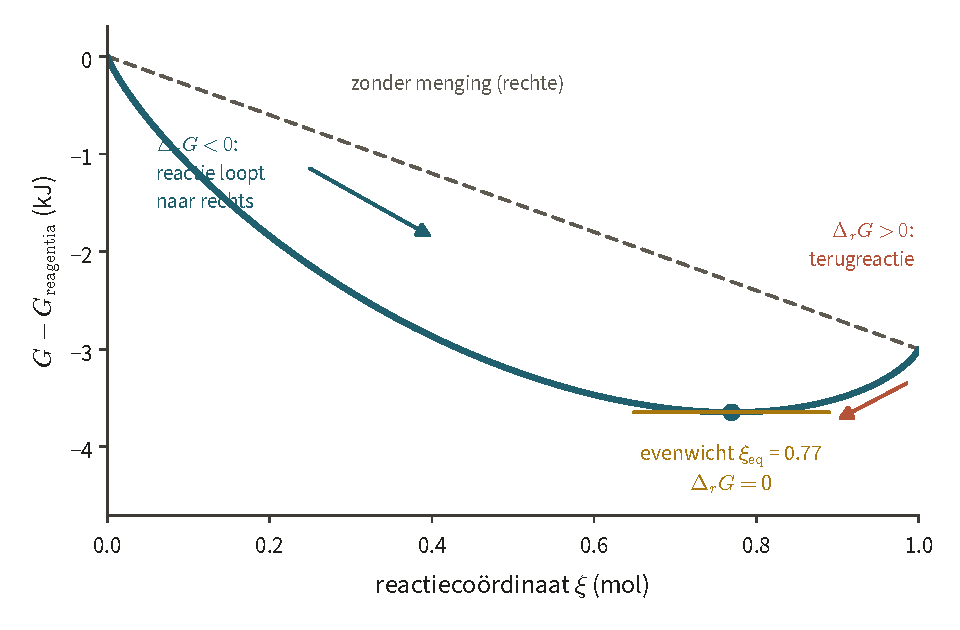
\includegraphics[width=0.7\linewidth]{Figuren/g_reactiecoordinaat}
    \caption{Gibbs-vrije energie van een ideaal gasmengsel $\mathrm{A}\rightleftharpoons\mathrm{B}$ ($\Delta_rG^\circ=\SI{-3}{\kilo\joule\per\mole}$, \SI{298}{\kelvin}) in functie van de reactiecoördinaat $\xi$. Zonder menging zou $G$ lineair dalen tot zuiver B (stippellijn); de mengentropie trekt de curve omlaag en legt het minimum bij $\xi_{\text{eq}}=0.77$, waar de raaklijn horizontaal is ($\Delta_rG=\partial G/\partial\xi=0$). Links ervan verloopt de reactie spontaan naar rechts, rechts ervan verloopt de terugreactie.}
    \label{fig:G-reactiecoordinaat}
\end{figure}

\subsection{Standaardtoestanden per fase}
\label{sec:standaardtoestanden-reagerend}

We schrijven elke chemische potentiaal als $\mu_i = \mu_i^\circ + RT \ln a_i$ (hoofdstuk~\ref{ch:niet-reagerend}, \S~\ref{sec:activiteit}). De standaardtoestand, en dus de vorm van $a_i$, hangt af van de fase:
\begin{itemize}
\item \textbf{gas}: ideaal gas bij $p^\circ = \SI{1}{\bar}$, dus $a_i \approx p_i/p^\circ = y_i P/p^\circ$;
\item \textbf{zuivere vloeistof of vaste stof}: de zuivere stof, dus $a_i \approx 1$;
\item \textbf{opgeloste stof}: een ideale oplossing van $c^\circ = \SI{1}{\mole\per\litre}$, dus $a_i = \gamma_i\,c_i/c^\circ$.
\end{itemize}
Voor een opgeloste stof is de verdunde oplossing de natuurlijke referentie (de logica van Henry, \S~\ref{sec:henry}); voor een zuivere fase de zuivere stof (Raoult). Dat zuivere vaste stoffen en vloeistoffen $a = 1$ hebben, vereenvoudigt heterogene evenwichten sterk (\S~\ref{sec:heterogene-evenwichten}).

\subsection{Het reactiequoti\"ent en de evenwichtsconstante}
\label{sec:evenwichtsconstante-reagerend}\label{sec:evenwichtsconstante}

Vul $\mu_i = \mu_i^\circ + RT \ln a_i$ in in vergelijking~\eqref{eq:delta-r-G}:
\begin{equation}
\Delta_r G = \Delta_r G^\circ + RT \ln Q,
\qquad
\Delta_r G^\circ = \sum_i \nu_i \mu_i^\circ,
\qquad
Q = \prod_i a_i^{\nu_i}.
\end{equation}
$\Delta_r G^\circ$ hangt enkel van de temperatuur af; het \emph{reactiequoti\"ent} $Q$ verandert terwijl de reactie loopt. In evenwicht is $\Delta_r G = 0$ en $Q = K$:
\begin{equation}
\boxed{\;\Delta_r G^\circ = -RT \ln K\;}
\label{eq:K-uit-drG}
\end{equation}
Zo kan je ook schrijven $\Delta_rG = RT\ln(Q/K)$: zolang $Q < K$ loopt de reactie vooruit, bij $Q > K$ achteruit. Elke \SI{5.7}{\kilo\joule\per\mole} in $\Delta_rG^\circ$ verschuift $K$ bij \SI{298}{\kelvin} met een factor tien.

\subsection{Berekening van $\Delta_rG^\circ$ en $K$ uit tabelwaarden}
\label{sec:drG-uit-tabellen}

Er zijn twee equivalente routes, net als voor $\Delta_rH^\circ$ (hoofdstuk~\ref{ch:energie}):
\begin{equation}
\Delta_r G^\circ = \sum_i \nu_i\,\Delta_fG_i^\circ
\qquad\text{of}\qquad
\Delta_rG^\circ = \Delta_rH^\circ - T\,\Delta_rS^\circ,
\end{equation}
met $\Delta_fG^\circ$ de \emph{standaardvormings-Gibbsenergie} (nul voor elementen in hun standaardtoestand).

\begin{voorbeeld}{$K$ voor de ammoniaksynthese bij \SI{298}{\kelvin}}
Route 1: $\Delta_fG^\circ(\mathrm{NH_3,g}) = \SI{-16.4}{\kilo\joule\per\mole}$, dus $\Delta_rG^\circ = 2(-16.4) = \SI{-32.8}{\kilo\joule\per\mole}$.

Route 2: $\Delta_rG^\circ = -92\,000 - 298.15 \times (-198.1) = \SI{-32.9}{\kilo\joule\per\mole}$ ($\Delta_rS^\circ$ uit hoofdstuk~\ref{ch:spontaniteit}, \S~\ref{sec:derde-hoofdwet}).

Beide routes geven hetzelfde, zoals het hoort. Dan is
\[
\ln K = -\frac{-32\,900}{8.314 \times 298.15} = 13.3 \quad\Rightarrow\quad K \approx 6\times10^{5}.
\]
Bij kamertemperatuur is ammoniak dus sterk bevoordeeld. Waarom dan toch \SI{450}{\celsius}? Zie verder.
\end{voorbeeld}

\subsection{Invloed van de temperatuur: de vergelijking van Van 't Hoff}
\label{sec:vanthoff}\label{sec:vanthoff-reagerend}

Hoe $K$ met $T$ verandert, volgt uit de \emph{Gibbs--Helmholtzvergelijking}. Met $(\partial G/\partial T)_p = -S$ (vergelijking~\eqref{eq:fundG}) en $G = H - TS$ geeft de quoti\"entregel
\begin{equation}
\left(\frac{\partial (G/T)}{\partial T}\right)_p = -\frac{S}{T} - \frac{G}{T^2} = -\frac{H}{T^2}.
\label{eq:gibbs-helmholtz}
\end{equation}
Pas dit toe op $\Delta_rG^\circ/T = -R\ln K$, en je krijgt de \emph{vergelijking van Van 't Hoff}:
\begin{gather}
\frac{\dd{\ln K}}{\dd T} = \frac{\Delta_r H^\circ}{RT^2}
\label{eq:vanthoff-diff}\\
\boxed{\;\ln\frac{K_2}{K_1} = -\frac{\Delta_rH^\circ}{R}\left(\frac{1}{T_2}-\frac{1}{T_1}\right)\;}
\label{eq:vanthoff-int}
\end{gather}
De tweede vorm veronderstelt $\Delta_rH^\circ$ constant. Een exotherme reactie verliest dus $K$ bij opwarmen, een endotherme wint. Figuur~\ref{fig:K-temperatuur} toont dat voor vijf industri\"ele reacties: wie de grafiek kent, weet meteen waarom stoomreforming heet moet en waarom de SO$_3$-reactor gekoeld wordt.

\begin{figure}[htb]
    \centering
    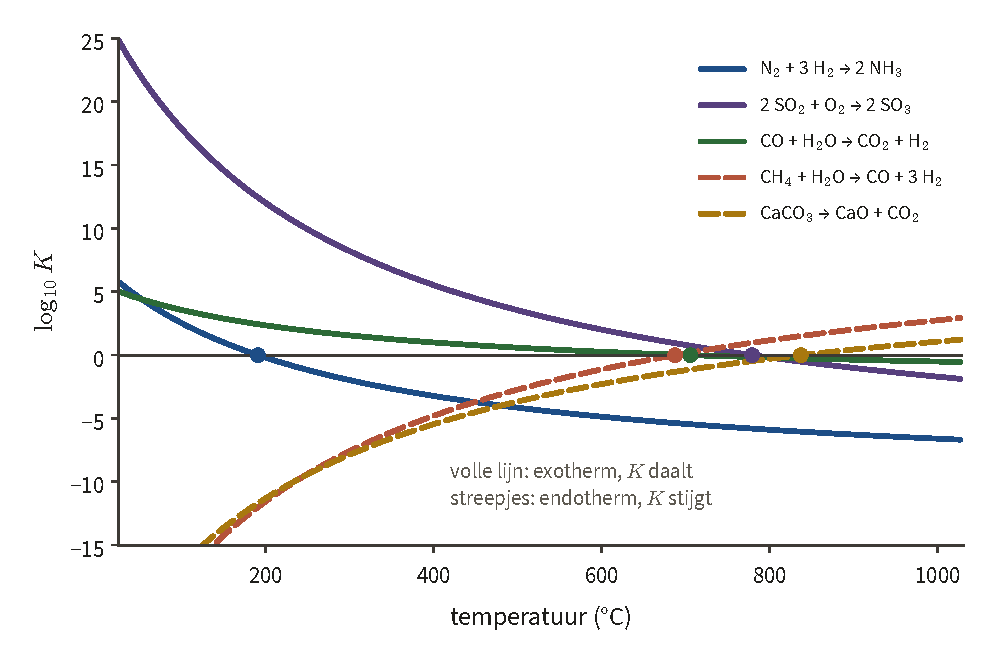
\includegraphics[width=0.75\linewidth]{Figuren/K_temperatuur}
    \caption{Evenwichtsconstante van vijf industri\"ele reacties in functie van de temperatuur, berekend met $\Delta_rH^\circ$ en $\Delta_rS^\circ$ bij \SI{298}{\kelvin} (constant verondersteld; bron: NIST WebBook). Het punt op de horizontale lijn $K = 1$ ligt bij $T = \Delta_rH^\circ/\Delta_rS^\circ$. Exotherme reacties (volle lijn) worden ongunstiger bij hoge $T$, endotherme (streepjes) gunstiger.}
    \label{fig:K-temperatuur}
\end{figure}

\begin{voorbeeld}{Ammoniak bij \SI{700}{\kelvin}}
Met $K_1 = 6\times10^5$ bij \SI{298.15}{\kelvin}:
\[
\ln\frac{K_2}{K_1} = \frac{92\,000}{8.314}\left(\frac{1}{700}-\frac{1}{298.15}\right) = -21.3
\quad\Rightarrow\quad K_2 \approx 3\times10^{-4}.
\]
Tien grootteordes minder (figuur~\ref{fig:vanthoff}). Bij \SI{700}{\kelvin} is de reactie thermodynamisch ongunstig. Dat men toch zo warm werkt, is een keuze voor snelheid (hoofdstuk~\ref{ch:kinetiek}); de hoge druk moet de opbrengst terugwinnen (\S~\ref{sec:ice-tabel}).
\end{voorbeeld}

\begin{figure}[htb]
    \centering
    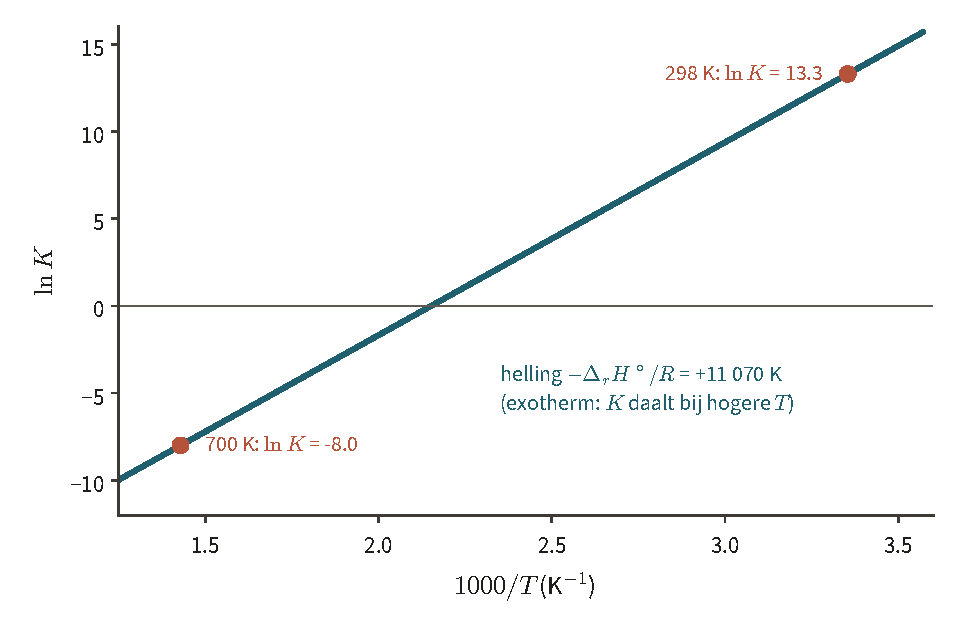
\includegraphics[width=0.65\linewidth]{Figuren/vanthoff_ammoniak}
    \caption{Van 't Hoff-diagram voor de ammoniaksynthese, met $\Delta_rH^\circ=\SI{-92}{\kilo\joule\per\mole}$ constant verondersteld en de twee punten uit het voorbeeld. Omdat de reactie exotherm is, stijgt $\ln K$ met $1/T$: de evenwichtsconstante daalt bij hogere temperatuur. De helling is $-\Delta_rH^\circ/R$ (vergelijking~\eqref{eq:vanthoff-int}).}
    \label{fig:vanthoff}
\end{figure}

\subsection{Verband tussen $K_p$, $K_c$ en $K_x$}
\label{sec:Kp-Kc-Kx}

Voor gasreacties kan je $K$ uitdrukken met parti\"ele drukken ($K_p$), concentraties ($K_c$) of molfracties ($K_x$). Met $p_i = y_i P = c_i RT$ voor ideale gassen:
\begin{equation}
K_p = K_c \left(\frac{RT}{p^\circ}\right)^{\Delta \nu} = K_x \left(\frac{P}{p^\circ}\right)^{\Delta \nu},
\label{eq:Kp-Kc-Kx-relatie}
\end{equation}
met $\Delta \nu$ de verandering van het aantal mol gas. $K_p$ en $K_c$ hangen enkel van $T$ af, $K_x$ ook van de totale druk. Voor ammoniak is $\Delta\nu = -2$, dus $K_x = K_p (P/p^\circ)^2$: honderd keer meer druk geeft $K_x$ tienduizend keer groter. Zo duwt druk het evenwicht naar ammoniak zonder $K_p$ te veranderen.

\section{Het chemisch evenwicht kwantitatief berekenen}

\subsection{Numerieke evenwichtsberekening met reactietabel (ICE-table)}
\label{sec:ice-tabel}

Het werkpaard van de ingenieur is de \emph{reactietabel} (ICE: Initial, Change, Equilibrium). Alle molhoeveelheden worden uitgedrukt in \'e\'en onbekende, $\xi$. Voor ammoniak met een stoichiometrische voeding:

\begin{center}
\begin{tabular}{lcccc}
\toprule
 & $\mathrm{N_2}$ & $\mathrm{H_2}$ & $\mathrm{NH_3}$ & totaal \\
\midrule
Initieel (mol) & 1 & 3 & 0 & 4 \\
Verandering (mol) & $-\xi$ & $-3\xi$ & $+2\xi$ & $-2\xi$ \\
Evenwicht (mol) & $1-\xi$ & $3-3\xi$ & $2\xi$ & $4-2\xi$ \\
\bottomrule
\end{tabular}
\end{center}
Met $p_i = y_i P$ en $y_i = n_i/n_\text{tot}$ wordt $K_p$ een functie van $\xi$ alleen, op te lossen met Doelzoeken in Excel.

\begin{voorbeeld}{Ammoniak bij \SI{700}{\kelvin} en \SI{100}{\bar}}
Met $K_p \approx 3\times10^{-4}$ (\S~\ref{sec:vanthoff}):
\[
K_p = \frac{\left(\dfrac{2\xi}{4-2\xi}\right)^2}{\left(\dfrac{1-\xi}{4-2\xi}\right)\left(\dfrac{3-3\xi}{4-2\xi}\right)^3}\left(\frac{P}{p^\circ}\right)^{-2} = 3\times10^{-4}
\quad\Rightarrow\quad \xi \approx 0.445.
\]
Het evenwichtsmengsel bevat $y_{\mathrm{NH_3}} = 0.891/3.109 = \SI{28.6}{\percent}$ ammoniak, en \SI{44.5}{\percent} van de stikstof is omgezet. Herhaal je dat voor andere drukken, dan krijg je figuur~\ref{fig:nh3-vs-druk}: bij \SI{1}{\bar} amper \SI{0.6}{\percent}, bij \SI{300}{\bar} bijna de helft.
\end{voorbeeld}

\begin{figure}[htb]
    \centering
    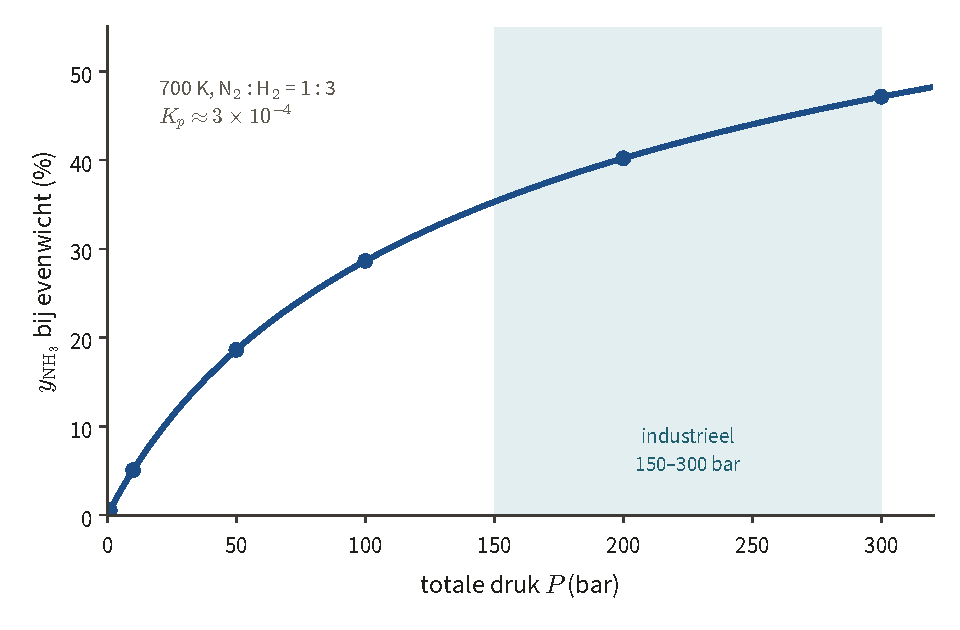
\includegraphics[width=0.7\linewidth]{Figuren/nh3_druk}
    \caption{Evenwichtsmolfractie ammoniak bij \SI{700}{\kelvin} in functie van de totale druk, voor een stoichiometrische voeding, berekend met de reactietabel. De opbrengst stijgt eerst snel en vlakt daarna af; de band toont het industri\"ele drukbereik.}
    \label{fig:nh3-vs-druk}
\end{figure}

\section{Factoren die het evenwicht be\"invloeden}

\subsection{Invloed van druk en inerte gassen}
\label{sec:druk-inerte-gassen}

\textbf{Druk} verandert $K_p$ niet, maar wel $K_x = K_p (P/p^\circ)^{-\Delta\nu}$ (\S~\ref{sec:Kp-Kc-Kx}). Bij $\Delta\nu < 0$ (ammoniak, methanol) helpt druk, bij $\Delta\nu > 0$ (stoomreforming) werkt ze tegen, bij $\Delta\nu = 0$ (watergasshift) maakt ze niets uit.

\textbf{Inerte gassen} (argon en methaan in de ammoniaklus) doen bij constante totale druk hetzelfde als een lagere druk: ze verdunnen de reagentia. Bij $\Delta\nu < 0$ daalt de opbrengst. Daarom spuit men in een recyclelus voortdurend een kleine \emph{purge} af, anders stapelen de inerten zich op (\S~\ref{sec:haber-bosch-integraal}).

\subsection{Het principe van Le Ch\^atelier}
\label{sec:le-chatelier-reagerend}\label{sec:le-chatelier}

Een verstoord evenwicht verschuift zo dat de verstoring deels wordt tegengewerkt:
opwarmen bevoordeelt de endotherme richting; druk verhogen de kant met minder mol gas; een product wegnemen of een reagens toevoegen bevoordeelt de producten. Dat is geen extra natuurwet: de verstoring verandert $G$ van alle toestanden, en het minimum schuift op. Van 't Hoff en $K_x$ maken het kwantitatief.

\subsection{Heterogene evenwichten}
\label{sec:heterogene-evenwichten}

Zuivere vaste stoffen en vloeistoffen hebben $a \approx 1$ en verdwijnen uit $K$.

\begin{voorbeeld}{Ontleding van kalksteen}
Voor $\mathrm{CaCO_3(s) \rightleftharpoons CaO(s) + CO_2(g)}$ is $K = p_{\mathrm{CO_2}}/p^\circ$. Bij elke temperatuur hoort dus \'e\'en evenwichtsdruk van \ce{CO2}, ongeacht hoeveel kalk er ligt: bij \SI{800}{\celsius} ongeveer \SI{0.22}{\bar}. Een kalkoven werkt alleen als de \ce{CO2}-druk boven de kalk lager blijft; daarom blaast men er rookgas of lucht door.
\end{voorbeeld}

Hetzelfde geldt voor het oplossen van een zout: voor $\mathrm{AgCl(s) \rightleftharpoons Ag^+ + Cl^-}$ is $K_{ps} = a_{\mathrm{Ag^+}}a_{\mathrm{Cl^-}} = 1.8\times10^{-10}$ bij \SI{25}{\celsius}, zodat $s = \sqrt{K_{ps}} = \SI{1.3e-5}{\mole\per\litre}$ (meer hierover in Analytische chemie).

\subsection{Gekoppelde reacties en simultane evenwichten}
\label{sec:gekoppelde-reacties}

Vaak lopen meerdere reacties tegelijk, met gemeenschappelijke componenten. Dan moet het mengsel aan elke evenwichtsvoorwaarde tegelijk voldoen, met een reactie-uitbreiding $\xi_1$, $\xi_2$, \ldots\ per reactie. Dat is de ICE-methode met meer onbekenden; in de praktijk lost een processimulator dit op. Het belangrijkste voorbeeld is de productie van waterstof.

\subsection{Tweede case: waterstof uit aardgas}
\label{sec:case-waterstof}

De waterstof voor ammoniak komt grotendeels uit aardgas, via twee gekoppelde evenwichten met een tegengesteld karakter (figuur~\ref{fig:K-temperatuur}).

\paragraph{Stoomreforming: endotherm, dus heet.}
\[
\ce{CH4 + H2O <=> CO + 3 H2}, \qquad \Delta_r H^\circ = \SI{+206}{\kilo\joule\per\mole},\quad \Delta\nu = +2.
\]
Hoge temperatuur en lage druk zijn gunstig. Men werkt bij \SIrange{800}{900}{\celsius} in buizen met nikkelkatalysator, van buitenaf verwarmd in een oven. De druk is toch \SIrange{20}{30}{\bar}: de rest van de installatie werkt onder druk, en een compacte reactor is goedkoper, ook al kost dat wat omzetting.

\paragraph{Watergasshift: exotherm, dus in twee trappen.}
\[
\ce{CO + H2O <=> CO2 + H2}, \qquad \Delta_r H^\circ = \SI{-41.2}{\kilo\joule\per\mole},\quad \Delta_r S^\circ = \SI{-42.1}{\joule\per\mole\per\kelvin},\quad \Delta\nu = 0.
\]

\begin{voorbeeld}{Watergasshift bij 400 en \SI{200}{\celsius}}
Voeding: 1 mol \ce{CO} en 2 mol \ce{H2O}. Bij omzetting $X$ is (druk en totaal aantal mol vallen weg, want $\Delta\nu = 0$):
\[
K = \frac{X^2}{(1-X)(2-X)}.
\]
\textbf{Bij \SI{400}{\celsius}}: $\ln K = 41\,200/(8.314 \times 673) - 42.1/8.314 = 7.36 - 5.06 = 2.30$, dus $K \approx 10$ en $9X^2 - 30X + 20 = 0$ geeft $X = 0.92$.

\textbf{Bij \SI{200}{\celsius}}: $\ln K = 10.48 - 5.06 = 5.41$, dus $K \approx 220$ en $X = 0.995$.

Bij \SI{400}{\celsius} blijft 8\,\% CO over, bij \SI{200}{\celsius} nog 0.5\,\%. Daarom twee shiftreactoren na elkaar: een \emph{hogetemperatuurshift} (\SIrange{350}{450}{\celsius}, ijzer-chroom) die snel het grootste deel omzet, en na tussenkoeling een \emph{lagetemperatuurshift} (\SIrange{200}{250}{\celsius}, koper) die het evenwicht verder duwt. De thermodynamica wil koud, de kinetiek warm: de ingenieur splitst het probleem op.
\end{voorbeeld}

\section{Van thermodynamica naar procesontwerp}

\subsection{Thermodynamische strategie\"en voor procesontwerp}
\label{sec:procesontwerp-strategieen}

De thermodynamica bepaalt de maximale omzetting; het procesontwerp bepaalt hoe dicht je erbij komt. Vier strategie\"en volgen rechtstreeks uit dit hoofdstuk:
\begin{enumerate}
\item \textbf{Temperatuur en druk kiezen} met Van 't Hoff en $K_x$.
\item \textbf{Product verwijderen}: houdt $Q < K$, zodat de reactie blijft lopen zonder dat $K$ verandert. Ammoniak wordt na afkoeling gecondenseerd; bij een verestering haalt men het water weg.
\item \textbf{Recycleren}: wat per doorgang niet reageert (bij ammoniak meer dan de helft), wordt na scheiding teruggestuurd, met een purge voor de inerten.
\item \textbf{Reactie en scheiding integreren}: reactieve destillatie, membraanreactoren. Het product verdwijnt al tijdens de reactie.
\end{enumerate}

\subsection{Evenwicht en warmte samen: de adiabatische reactor}
\label{sec:adiabatische-evenwichtsreactor}

In een adiabatische reactor warmt een exotherme reactie het mengsel op: $T = T_\mathrm{in} + \Delta T_\mathrm{ad}\,X$ (hoofdstuk~\ref{ch:energie}, \S~\ref{sec:warmte-effecten}). Bij een evenwichtsreactie is dat vervelend: hoe meer omzetting, hoe warmer, hoe lager de evenwichtsomzetting. De reactie stopt waar de rechte van de energiebalans de evenwichtscurve snijdt.

Figuur~\ref{fig:so2-bedden} toont dat voor $\ce{SO2 + 1/2 O2 <=> SO3}$ ($\Delta_r H^\circ = \SI{-98.9}{\kilo\joule\per\mole}$) in een zwavelzuurfabriek, met 10\,\% \ce{SO2}, 11\,\% \ce{O2} en 79\,\% \ce{N2}. Met een gemiddelde $C_p = \SI{32}{\joule\per\mole\per\kelvin}$ is $\Delta T_\mathrm{ad} = 0.10 \times 98\,900/32 \approx \SI{310}{\kelvin}$ bij volledige omzetting.

\begin{figure}[htb]
    \centering
    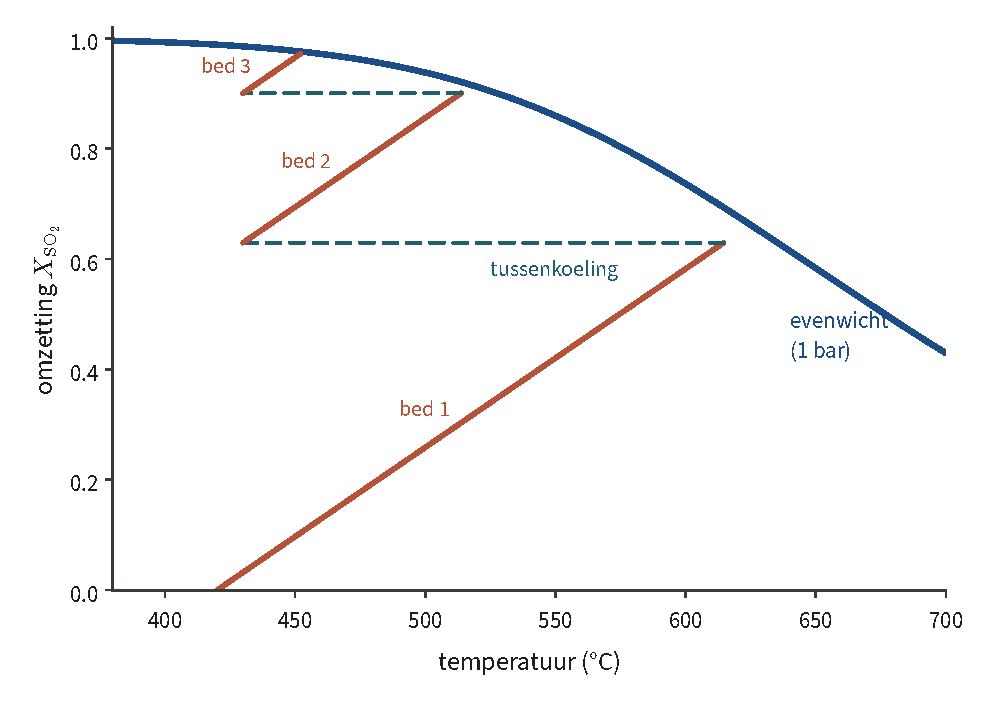
\includegraphics[width=0.75\linewidth]{Figuren/so2_bedden}
    \caption{Evenwichtsomzetting van \ce{SO2} naar \ce{SO3} (blauw) en drie adiabatische katalysatorbedden met tussenkoeling tot \SI{430}{\celsius} (rood). In elk bed stijgen omzetting en temperatuur samen langs een rechte, tot dicht bij het evenwicht. Berekend met $\Delta_r H^\circ$ en $\Delta_r S^\circ$ uit tabellen (NIST) en een gemiddelde $C_p$.}
    \label{fig:so2-bedden}
\end{figure}

Het eerste bed start bij \SI{420}{\celsius} (kouder werkt de vanadiumkatalysator niet) en loopt op tot ongeveer \SI{615}{\celsius} bij 63\,\% omzetting. Na afkoeling tot \SI{430}{\celsius} brengt een tweede bed de omzetting naar 90\,\%, een derde naar 97\,\%. Moderne installaties absorberen dan het \ce{SO3} en sturen het restgas door een vierde bed (\emph{dubbele absorptie}): product weg, $Q$ omlaag, meer dan 99.7\,\%. Met de warmte uit de tussenkoelers maakt men stoom: een zwavelzuurfabriek levert netto energie.

\subsection{Ge\"integreerde casestudy: de synthese van ammoniak}
\label{sec:haber-bosch-integraal}

We kunnen nu de drie vragen uit \S~\ref{sec:haber-bosch} beantwoorden (figuur~\ref{fig:haber-bosch-schema}).

\begin{figure}[htb]
    \centering
    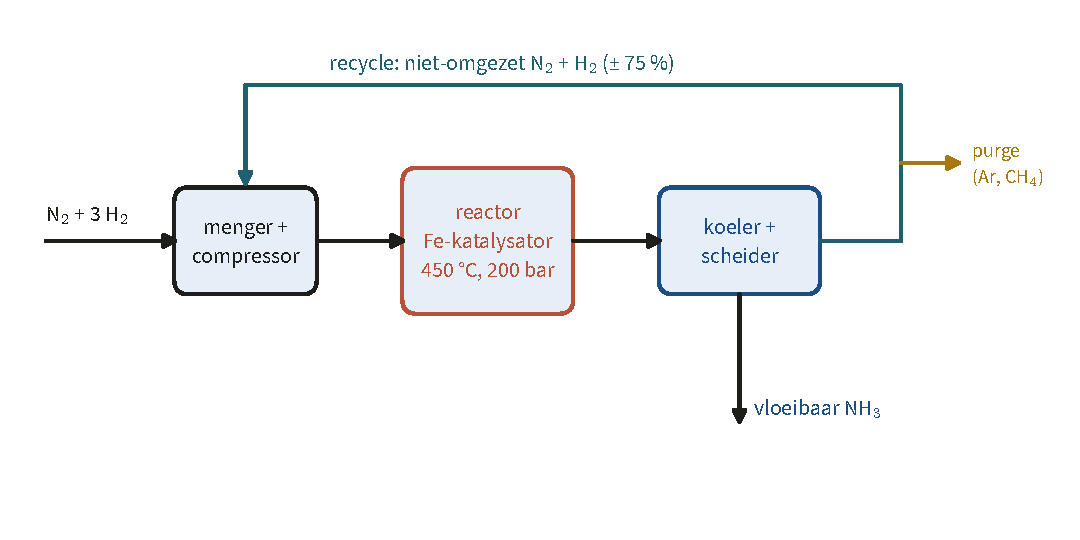
\includegraphics[width=0.85\linewidth]{Figuren/haber_bosch_schema}
    \caption{Vereenvoudigd blokschema van de Haber--Boschlus. Per doorgang wordt slechts een deel van \ce{N2} en \ce{H2} omgezet; na afkoeling condenseert \ce{NH3} en wordt het afgescheiden. De rest gaat terug naar de reactor (recycle), met een kleine purge om inerte gassen af te voeren.}
    \label{fig:haber-bosch-schema}
\end{figure}

\begin{itemize}
\item \textbf{Waarom stopt de reactie halfweg?} Het minimum van $G$ ligt tussen reagentia en producten (figuur~\ref{fig:G-reactiecoordinaat}).
\item \textbf{Waarom \SI{450}{\celsius}?} Bij kamertemperatuur is $K = 6\times10^5$, maar de $\mathrm{N{\equiv}N}$-binding maakt de reactie veel te traag. Warmer gaat sneller, maar $K$ daalt tot $3\times10^{-4}$ bij \SI{700}{\kelvin}. Een ijzerkatalysator verlaagt de nodige temperatuur, zonder $K$ te veranderen (hoofdstuk~\ref{ch:kinetiek}).
\item \textbf{Waarom \SIrange{150}{300}{\bar}?} Omdat $\Delta\nu = -2$: druk wint de opbrengst terug die de temperatuur kost (figuur~\ref{fig:nh3-vs-druk}).
\item \textbf{Hoeveel ammoniak?} Per doorgang zet men minder dan de helft om. Ammoniak condenseren en het restgas recycleren (met purge) brengt de globale omzetting toch boven \SI{95}{\percent}.
\end{itemize}

\begin{besluit}{Thermodynamica bepaalt, kinetiek levert}
De thermodynamica legt de grens vast; het werkpunt van een installatie is een compromis tussen evenwicht, snelheid, energie, investering en veiligheid.
\end{besluit}

\section{Samenvatting en reflectie}

Het criterium van hoofdstuk~\ref{ch:spontaniteit}, een minimale Gibbs-vrije energie, bepaalt ook waar een chemische reactie stopt. In hoofdstuk~\ref{ch:elektrochemie} breiden we dit uit naar systemen waarin naast de chemische potentiaal ook de elektrische potentiaal een rol speelt: batterijen, brandstofcellen, elektrolysers en corrosie.

\begin{samenvatting}{Thermodynamisch evenwicht van reagerende systemen}
\begin{itemize}
\item De reactie-Gibbsenergie $\Delta_rG=\sum_i\nu_i\mu_i$ is de helling van $G$ langs de reactieco\"ordinaat $\xi$; evenwicht ligt in het minimum, waar $\Delta_rG=0$.
\item Met $\mu_i=\mu_i^\circ+RT\ln a_i$ volgt $\Delta_rG=\Delta_rG^\circ+RT\ln Q$ en in evenwicht $\Delta_rG^\circ=-RT\ln K$. $Q<K$: de reactie loopt vooruit.
\item $\Delta_rG^\circ$ volgt uit tabellen: $\sum_i\nu_i\Delta_fG_i^\circ$ of $\Delta_rH^\circ-T\Delta_rS^\circ$.
\item Van 't Hoff: $\dd\ln K/\dd T=\Delta_rH^\circ/RT^2$. Exotherme reacties verliezen opbrengst bij hogere temperatuur.
\item $K_p$ en $K_c$ hangen enkel van $T$ af; $K_x=K_p(P/p^\circ)^{-\Delta\nu}$ hangt ook van de druk af. Inerte gassen verlagen bij constante druk de opbrengst van reacties met $\Delta\nu<0$.
\item De evenwichtssamenstelling volgt uit een reactietabel en \'e\'en vergelijking in $\xi$ (of meerdere, bij gekoppelde reacties).
\item Zuivere vaste stoffen en vloeistoffen hebben activiteit 1 en verschijnen niet in $K$.
\item In een adiabatische reactor stijgt de temperatuur met de omzetting (werklijn) tot ze de evenwichtscurve snijdt. Bij exotherme evenwichtsreacties (SO$_2$-oxidatie, watergasshift) werkt men daarom met meerdere bedden en tussenkoeling: eerst snelheid bij hoge $T$, dan opbrengst bij lage $T$.
\item Ontwerpstrategie\"en: $T$ en $P$ kiezen, product verwijderen, recycleren met purge, reactie en scheiding integreren. Thermodynamica bepaalt de grens, kinetiek en economie het werkpunt.
\end{itemize}
\end{samenvatting}

\begin{reflectie}{Thermodynamisch evenwicht van reagerende systemen}
\begin{enumerate}
\item Waarom stopt een reactie in een gesloten vat meestal v\'o\'or alle reagentia op zijn, ook als $\Delta_rG^\circ$ sterk negatief is?
\item Een katalysator verlaagt de activeringsenergie. Waarom verandert hij $K$ niet?
\item Waarom heeft een drukverhoging geen invloed op $K_p$, maar wel op de opbrengst van ammoniak?
\item Bij de ammoniaksynthese daalt $K$ met tien grootteordes tussen \SI{298}{\kelvin} en \SI{700}{\kelvin}. Waarom werkt men toch bij \SI{700}{\kelvin}?
\item Waarom haalt een groter adiabatisch katalysatorbed niet altijd een hogere omzetting?
\item Wat gebeurt er met de reactorcapaciteit als je de purge in de Haber--Boschlus dichtdraait?
\item Een kalkoven werkt bij atmosferische druk. Waarom blaast men lucht of rookgas door de oven?
\item Geef een voorbeeld van een proces waarin reactie en scheiding in \'e\'en toestel gebeuren, en leg uit waarom dat de omzetting verhoogt.
\end{enumerate}
\end{reflectie}

\newpage
\section{Oefeningen}

% Oefeningen bij dit hoofdstuk (ingevoegd achteraan het hoofdstuk met \input).
% Een oefening:  \begin{oefening}[titel] ... \end{oefening}   (boek en website)
% De oplossing:  \begin{oplossing} ... \end{oplossing}       (enkel website, dichtgeklapt)

Neem $R = \SI{8.314}{\joule\per\mole\per\kelvin}$, $p^\circ = \SI{1}{\bar}$ en $c^\circ = \SI{1}{\mole\per\litre}$; gassen zijn ideaal.

\begin{oefening}[Evenwichtsconstante en standaardreactie-Gibbsenergie]
Voor de reactie

\[
\mathrm{N_2O_4(g) \rightleftharpoons 2\,NO_2(g)}
\]

bedraagt \(\Delta_r G^\circ = +4.8\,\mathrm{kJ/mol}\) bij \(298\,\mathrm{K}\).

\begin{enumerate}
\item[(a)]
  Bereken de evenwichtsconstante \(K\) bij \(298\,\mathrm{K}\).
\item[(b)]
  Is de reactie bij standaardomstandigheden spontaan in de voorwaartse richting?
\item[(c)]
  Bij welke waarde van het reactiequotiënt \(Q\) zou de reactie precies in evenwicht zijn?
\end{enumerate}
\end{oefening}
\begin{oplossing}
\textbf{Resultaat:} (a) \(K\) = \textbf{0.144}. (b) \textbf{Nee}, bij \(Q = 1\) verloopt de reactie naar links. (c) Evenwicht bij \(Q = K\) = \textbf{0.144}.

\textbf{(a)} \(K = \exp(-\Delta_r G^\circ/RT) = \exp\!\left(-\dfrac{4800}{(8.314)(298)}\right) = 0.144\).

\textbf{(b)} Nee. Bij standaardomstandigheden (beide gassen bij \(1\,\mathrm{bar}\), dus \(Q = 1\)) is \(\Delta_r G = \Delta_r G^\circ > 0\): de reactie verloopt spontaan in de \emph{omgekeerde} richting tot het evenwicht bereikt is. Dat betekent niet dat er geen \(\mathrm{NO_2}\) gevormd wordt: vertrekkend van zuiver \(\mathrm{N_2O_4}\) (\(Q = 0\)) dissocieert een deel wel degelijk.

\textbf{(c)} Evenwicht wanneer \(\Delta_r G = \Delta_r G^\circ + RT\ln Q = 0\), dus \(Q = K = 0.144\).
\end{oplossing}

\begin{oefening}[Invloed van temperatuur: de vergelijking van Van 't Hoff]
Voor de ammoniaksynthese \(\mathrm{N_2 + 3\,H_2 \rightleftharpoons 2\,NH_3}\) bedraagt \(\Delta_r H^\circ = -92.4\,\mathrm{kJ/mol}\) en \(\Delta_r G^\circ = -33.0\,\mathrm{kJ/mol}\) bij \(298\,\mathrm{K}\).

\begin{enumerate}
\item[(a)]
  Bereken \(K\) bij \(298\,\mathrm{K}\).
\item[(b)]
  Schat \(K\) bij \(700\,\mathrm{K}\) (veronderstel \(\Delta_r H^\circ\) constant). Gebruik de geïntegreerde vorm van Van 't Hoff.
\item[(c)]
  Verklaar vanuit het teken van \(\Delta_r H^\circ\) waarom de evenwichtsconstante daalt bij stijgende temperatuur.
\item[(d)]
  Combineer met Hoofdstuk 1: bereken ook \(\Delta_r S^\circ\) bij \(298\,\mathrm{K}\).
\end{enumerate}
\end{oefening}
\begin{oplossing}
\textbf{Resultaat:} (a) \(K_{298}\) = \textbf{6.1\ensuremath{\cdot{}}10\ensuremath{^{5}}}. (b) \(K_{700}\) = \textbf{3.0\ensuremath{\cdot{}}10\ensuremath{^{-4}}}. (c) Exotherm: \(K\) \textbf{daalt} met \(T\). (d) \(\Delta_r S^\circ\) = \textbf{\ensuremath{-}199 J/(mol\ensuremath{\cdot{}}K)}.

\textbf{(a)} \(\ln K = 33\,000/(8.314 \times 298) = 13.32\), dus \(K = 6.1\times10^{5}\).

\textbf{(b)}

\[
\ln\frac{K_2}{K_1} = -\frac{-92\,400}{8.314}\left(\frac{1}{700} - \frac{1}{298}\right) = -21.4
\]

zodat \(\ln K_2 = 13.32 - 21.4 = -8.1\) en \(K_2 = 3.0\times10^{-4}\).

\textbf{(c)} Volgens \(\mathrm{d}\ln K/\mathrm{d}T = \Delta_r H^\circ/(RT^2)\) daalt \(\ln K\) met \(T\) wanneer \(\Delta_r H^\circ < 0\). Fysisch: bij een exotherme reactie ``werkt'' extra warmte de vorming van producten tegen (Le Chatelier).

\textbf{(d)} \(\Delta_r S^\circ = (\Delta_r H^\circ - \Delta_r G^\circ)/T = (-92\,400 + 33\,000)/298 = -199\,\mathrm{J/(mol\cdot K)}\), in overeenstemming met de \(-198.1\,\mathrm{J/(mol\cdot K)}\) uit de theorie. Negatief, omdat 4 mol gas omgezet wordt in 2 mol gas.
\end{oplossing}

\begin{oefening}[Le Châtelier: invloed van druk op ammoniaksynthese]
Beschouw opnieuw de ammoniaksynthese. Bij een bepaalde temperatuur bedraagt \(K = 1.0\times10^{-3}\).

\begin{enumerate}
\item[(a)]
  Een reactiemengsel bevat aanvankelijk gelijke molfracties \(\mathrm{N_2}\), \(\mathrm{H_2}\) en \(\mathrm{NH_3}\) bij een totale druk van \(1\,\mathrm{bar}\). Bereken \(Q\) en bepaal de spontane richting.
\item[(b)]
  Hoe verandert \(Q\) wanneer de totale druk wordt verhoogd tot \(200\,\mathrm{bar}\)? Verklaar waarom een drukverhoging de vorming van ammoniak bevordert.
\item[(c)]
  Waarom verandert de evenwichtsconstante \(K\) zelf \emph{niet} met de druk?
\end{enumerate}

\emph{Hint:} bij een gasreactie met afname van aantal mol geldt \(Q \propto p^{\Delta \nu} = 1/p^{|\Delta \nu|}\).
\end{oefening}
\begin{oplossing}
\textbf{Resultaat:} (a) \(Q\) = \textbf{9} \textgreater{} \(K\): ammoniak ontleedt. (b) \(Q\) = \textbf{2.25\ensuremath{\cdot{}}10\ensuremath{^{-4}}} \textless{} \(K\): ammoniak wordt gevormd. (c) \(K\) hangt enkel af van \(T\).

\textbf{(a)} Met \(p_i = x_i p\) en \(p^\circ = 1\,\mathrm{bar}\):

\[
Q = \frac{(x_{\mathrm{NH_3}}p/p^\circ)^2}{(x_{\mathrm{N_2}}p/p^\circ)(x_{\mathrm{H_2}}p/p^\circ)^3} = \frac{x_{\mathrm{NH_3}}^2}{x_{\mathrm{N_2}}x_{\mathrm{H_2}}^3}\left(\frac{p}{p^\circ}\right)^{-2} = \frac{(1/3)^2}{(1/3)^4}(1)^{-2} = 9
\]

\(Q = 9 \gg K\): de reactie verloopt spontaan naar links, ammoniak ontleedt.

\textbf{(b)} De samenstelling blijft dezelfde, maar de drukfactor wordt \((200)^{-2}\): \(Q = 9/40\,000 = 2.25\times10^{-4} < K\). Nu verloopt de reactie spontaan naar rechts. Omdat het aantal mol gas afneemt (\(\Delta\nu = 2 - 4 = -2\)), daalt \(Q\) met de druk als \(p^{\Delta\nu} = p^{-2}\); het evenwicht moet dan naar de kant van de producten schuiven om \(Q\) weer gelijk te maken aan \(K\).

\textbf{(c)} \(K = \exp(-\Delta_r G^\circ/RT)\) is gedefinieerd met de standaardtoestand bij de vaste druk \(p^\circ = 1\,\mathrm{bar}\). Daardoor hangt \(K\) enkel af van de temperatuur. De druk verandert wel \(Q\), en dus de evenwichtssamenstelling.
\end{oplossing}

\begin{oefening}[\(K_p\), \(K_c\) en \(K_x\) voor de ammoniaksynthese]
Voor \(\mathrm{N_2 + 3\,H_2 \rightleftharpoons 2\,NH_3}\) geldt \(K_p \approx 3\times10^{-4}\) bij \(700\,\mathrm{K}\).

\begin{enumerate}
\item[(a)]
  Bereken \(K_c\) bij \(700\,\mathrm{K}\). Let op de eenheden: gebruik \(c^\circ = 1\,\mathrm{mol/L} = 1000\,\mathrm{mol/m^3}\).
\item[(b)]
  Bereken \(K_x\) bij \(1\,\mathrm{bar}\) en bij \(200\,\mathrm{bar}\).
\item[(c)]
  Welke van de drie constanten verandert wanneer je de reactor bij dezelfde temperatuur op een hogere druk zet? Waarom is \(K_c \neq K_p\)?
\end{enumerate}
\end{oefening}
\begin{oplossing}
\textbf{Resultaat:} (a) \(K_c\) \ensuremath{\approx{}} \textbf{1.0}. (b) \(K_x\) = \textbf{3\ensuremath{\cdot{}}10\ensuremath{^{-4}}} bij 1 bar en \textbf{12} bij 200 bar. (c) Enkel \textbf{\(K_x\)} verandert met de druk; \(K_c \neq K_p\) omdat \(\Delta\nu = -2 \neq 0\).

\textbf{(a)} Met \(p_i = c_i RT\) geldt \(K_p = K_c\,(c^\circ RT/p^\circ)^{\Delta\nu}\). Hier is

\[
\frac{c^\circ RT}{p^\circ} = \frac{(1000\,\mathrm{mol/m^3})(8.314)(700)}{10^5\,\mathrm{Pa}} = 58.2
\]

en \(\Delta\nu = -2\), dus \(K_c = K_p\,(58.2)^{2} = (3\times10^{-4})(3387) = 1.0\).

\textbf{(b)} \(K_x = K_p\,(P/p^\circ)^{-\Delta\nu} = K_p\,(P/p^\circ)^{2}\): bij \(1\,\mathrm{bar}\) is \(K_x = K_p = 3\times10^{-4}\), bij \(200\,\mathrm{bar}\) is \(K_x = 3\times10^{-4} \times 40\,000 = 12\).

\textbf{(c)} \(K_p\) en \(K_c\) hangen enkel van de temperatuur af; \(K_x\) groeit met \(P^2\), wat de hogere ammoniakfractie bij hoge druk verklaart. \(K_c\) en \(K_p\) verschillen omdat ze naar een andere standaardtoestand verwijzen (\(1\,\mathrm{mol/L}\) tegenover \(1\,\mathrm{bar}\)). Ze zijn enkel gelijk wanneer \(\Delta\nu = 0\), zoals bij de water-gas-shiftreactie.
\end{oplossing}

\begin{oefening}[Inert gas in de ammoniakreactor]
In het voorbeeld van \S~\ref{sec:ice-tabel} werd de evenwichtssamenstelling berekend bij \(700\,\mathrm{K}\) en \(100\,\mathrm{bar}\) (\(K_p \approx 3\times10^{-4}\)), vertrekkend van \(1\,\mathrm{mol}\) \(\mathrm{N_2}\) en \(3\,\mathrm{mol}\) \(\mathrm{H_2}\): \(\xi \approx 0.445\). In een echte installatie stapelt argon (uit de lucht) zich op in de recyclestroom.

\begin{enumerate}
\item[(a)]
  Stel de reactietabel op wanneer de voeding bovendien \(2\,\mathrm{mol}\) argon bevat, bij dezelfde totale druk van \(100\,\mathrm{bar}\).
\item[(b)]
  Bereken de omzetting van stikstof en de molfractie ammoniak. Vergelijk met de situatie zonder argon.
\item[(c)]
  Wat zou er gebeuren als je het argon toevoegt bij constant volume?
\item[(d)]
  Waarom voorziet men een purgestroom in de recyclelus?
\end{enumerate}
\end{oefening}
\begin{oplossing}
\textbf{Resultaat:} (b) \(\xi\) = \textbf{0.354} (35 \% omzetting, tegenover 44.5 \%); \(y_{\mathrm{NH_3}}\) = \textbf{0.134} (tegenover 0.286). (c) Bij constant volume: \textbf{geen effect}. (d) Zonder purge stapelt het inerte gas zich op en daalt de omzetting per doorgang.

\textbf{(a)}

\begin{center}
\begin{tabular}{lllll}
\toprule
 & \(\mathrm{N_2}\) & \(\mathrm{H_2}\) & \(\mathrm{NH_3}\) & Ar \\
\midrule
Initieel (mol) & 1 & 3 & 0 & 2 \\
Verandering (mol) & \(-\xi\) & \(-3\xi\) & \(+2\xi\) & 0 \\
Evenwicht (mol) & \(1-\xi\) & \(3-3\xi\) & \(2\xi\) & 2 \\
\bottomrule
\end{tabular}
\end{center}

met \(n_{\text{tot}} = 6 - 2\xi\).

\textbf{(b)} De evenwichtsvoorwaarde wordt

\[
K_p = \frac{\left(\dfrac{2\xi}{6-2\xi}\right)^2}{\left(\dfrac{1-\xi}{6-2\xi}\right)\left(\dfrac{3-3\xi}{6-2\xi}\right)^3}\left(\frac{P}{p^\circ}\right)^{-2} = 3\times10^{-4}
\]

Numeriek oplossen geeft \(\xi = 0.354\), \(n_{\text{tot}} = 5.29\,\mathrm{mol}\) en \(y_{\mathrm{NH_3}} = 0.708/5.29 = 0.134\). Zonder argon was \(\xi = 0.445\) en \(y_{\mathrm{NH_3}} = 0.286\). Het argon verdunt de reactanten: hun partiële drukken dalen, alsof de reactor bij een lagere druk werkt, en het evenwicht schuift naar de kant met meer mol gas.

\textbf{(c)} Bij constant volume blijven de partiële drukken van \(\mathrm{N_2}\), \(\mathrm{H_2}\) en \(\mathrm{NH_3}\) dezelfde; enkel de totale druk stijgt. \(Q\) verandert niet, dus het evenwicht verschuift niet.

\textbf{(d)} Bij elke doorgang wordt het ammoniak uitgecondenseerd en worden \(\mathrm{N_2}\) en \(\mathrm{H_2}\) teruggevoerd, maar het argon (en methaan) reageert niet en condenseert niet. Zonder purge zou de argonfractie blijven stijgen tot de reactor nauwelijks nog ammoniak maakt. Een kleine purgestroom houdt de inerte fractie op een paar procent; het verlies aan waterstof in die purge is de prijs die men betaalt.
\end{oplossing}

\begin{oefening}[Het bruine gas \(\mathrm{NO_2}\): druk en temperatuur]
Voor \(\mathrm{N_2O_4(g) \rightleftharpoons 2\,NO_2(g)}\) geldt \(K = 0.144\) bij \(298\,\mathrm{K}\) (Oefening 6.1) en \(\Delta_r H^\circ = +57.2\,\mathrm{kJ/mol}\). \(\mathrm{N_2O_4}\) is kleurloos, \(\mathrm{NO_2}\) roodbruin.

\begin{enumerate}
\item[(a)]
  Vertrek van zuiver \(\mathrm{N_2O_4}\) en noem \(\alpha\) de fractie die dissocieert. Toon aan dat \(K = \dfrac{4\alpha^2}{1-\alpha^2}\dfrac{P}{p^\circ}\).
\item[(b)]
  Bereken \(\alpha\) bij \(298\,\mathrm{K}\) en een totale druk van \(0.1\), \(1\) en \(10\,\mathrm{bar}\).
\item[(c)]
  Bereken \(K\) en \(\alpha\) bij \(350\,\mathrm{K}\) en \(1\,\mathrm{bar}\).
\item[(d)]
  Een afgesloten glazen buisje met dit gasmengsel wordt in ijswater en daarna in heet water gezet. Wat zie je? Verklaar met Le Châtelier.
\end{enumerate}
\end{oefening}
\begin{oplossing}
\textbf{Resultaat:} (b) \(\alpha\) = \textbf{0.51}, \textbf{0.19} en \textbf{0.06} bij 0.1, 1 en 10 bar. (c) \(K_{350}\) = \textbf{4.4}, \(\alpha\) = \textbf{0.73}. (d) Koud: bijna kleurloos; warm: \textbf{donkerbruin}.

\textbf{(a)} Per mol \(\mathrm{N_2O_4}\): bij evenwicht \(1-\alpha\) mol \(\mathrm{N_2O_4}\) en \(2\alpha\) mol \(\mathrm{NO_2}\), samen \(1+\alpha\) mol. Met \(p_i = y_iP\):

\[
K = \frac{\left(\dfrac{2\alpha}{1+\alpha}\right)^2}{\dfrac{1-\alpha}{1+\alpha}}\frac{P}{p^\circ} = \frac{4\alpha^2}{(1-\alpha)(1+\alpha)}\frac{P}{p^\circ} = \frac{4\alpha^2}{1-\alpha^2}\frac{P}{p^\circ}
\]

\textbf{(b)} Omvormen geeft \(\alpha = \sqrt{K/(K + 4P/p^\circ)}\):

\begin{center}
\begin{tabular}{llll}
\toprule
\(P\) (bar) & 0.1 & 1 & 10 \\
\midrule
\(\alpha\) & 0.51 & 0.19 & 0.06 \\
\bottomrule
\end{tabular}
\end{center}

Omdat \(\Delta\nu = +1\), duwt een hogere druk het evenwicht naar \(\mathrm{N_2O_4}\).

\textbf{(c)} Van 't Hoff:

\[
\ln\frac{K_{350}}{0.144} = -\frac{57\,200}{8.314}\left(\frac{1}{350} - \frac{1}{298}\right) = 3.43 \quad\Rightarrow\quad K_{350} = 4.4
\]

en \(\alpha = \sqrt{4.4/8.4} = 0.73\).

\textbf{(d)} De dissociatie is endotherm. In ijswater verschuift het evenwicht naar \(\mathrm{N_2O_4}\) en wordt het gas bijna kleurloos; in heet water naar \(\mathrm{NO_2}\) en wordt het donkerbruin. Dit is een klassieke demonstratie van Le Châtelier. \(\mathrm{NO_2}\) is ook het bruine gas in smog boven drukke wegen.
\end{oplossing}

\begin{oefening}[Bij welke temperatuur werkt een kalkoven?]
Voor \(\mathrm{CaCO_3(s) \rightleftharpoons CaO(s) + CO_2(g)}\) bedraagt de evenwichtsdruk van \(\mathrm{CO_2}\) \(0.22\,\mathrm{bar}\) bij \(800\,^\circ\mathrm{C}\) (voorbeeld in \S~\ref{sec:heterogene-evenwichten}). Neem \(\Delta_r H^\circ = +178.3\,\mathrm{kJ/mol}\) (Oefening 3.9), constant.

\begin{enumerate}
\item[(a)]
  Bereken de evenwichtsdruk van \(\mathrm{CO_2}\) bij \(900\,^\circ\mathrm{C}\).
\item[(b)]
  Bij welke temperatuur bereikt de ontbindingsdruk \(1\,\mathrm{bar}\)? Vergelijk met de temperatuur waarbij \(\Delta_r G^\circ = 0\) uit Oefening 3.9 (\(1110\,\mathrm{K}\)).
\item[(c)]
  Waarom blaast men lucht door een kalkoven, en waarom ontleedt kalksteen in een gesloten vat niet volledig?
\item[(d)]
  Hangt de evenwichtsdruk af van de hoeveelheid kalksteen in de oven?
\end{enumerate}
\end{oefening}
\begin{oplossing}
\textbf{Resultaat:} (a) \(p_{\mathrm{CO_2}}\) \ensuremath{\approx{}} \textbf{1.2 bar}. (b) \(T\) \ensuremath{\approx{}} \textbf{1161 K} (888 °C), ongeveer 50 K boven de schatting uit hoofdstuk 3. (c) Het weggeblazen CO\ensuremath{_{2}} houdt \textbf{\(Q < K\)}. (d) \textbf{Nee}: vaste stoffen hebben activiteit 1.

\textbf{(a)} Met \(K = p_{\mathrm{CO_2}}/p^\circ\) en Van 't Hoff:

\[
\ln\frac{K_{1173}}{0.22} = -\frac{178\,300}{8.314}\left(\frac{1}{1173.15} - \frac{1}{1073.15}\right) = 1.70 \quad\Rightarrow\quad K_{1173} = 1.2
\]

De evenwichtsdruk stijgt in \(100\,\mathrm{K}\) met een factor \(5.5\).

\textbf{(b)} \(K = 1\) wanneer

\[
\frac{1}{T} = \frac{1}{1073.15} - \frac{8.314}{178\,300}\ln\frac{1}{0.22} \quad\Rightarrow\quad T = 1161\,\mathrm{K} = 888\,^\circ\mathrm{C}
\]

\(K = 1\) betekent \(\Delta_r G^\circ = 0\): dit is dezelfde vraag als in Oefening 3.9. Daar vond je \(1110\,\mathrm{K}\) met \(\Delta_r H^\circ\) en \(\Delta_r S^\circ\) bij \(298\,\mathrm{K}\); het verschil van ongeveer \(50\,\mathrm{K}\) komt van de temperatuurafhankelijkheid van \(\Delta_r H^\circ\) en \(\Delta_r S^\circ\) (de wet van Kirchhoff). De experimentele waarde is ongeveer \(898\,^\circ\mathrm{C}\).

\textbf{(c)} Kalksteen ontleedt enkel zolang \(p_{\mathrm{CO_2}}\) in de oven onder de evenwichtsdruk blijft (\(Q < K\), dus \(\Delta_r G < 0\)). In een gesloten vat stijgt \(p_{\mathrm{CO_2}}\) tot de evenwichtsdruk en stopt de reactie. Door lucht of rookgas door de oven te blazen, wordt het \(\mathrm{CO_2}\) afgevoerd: productverwijdering uit \S~\ref{sec:procesontwerp-strategieen}.

\textbf{(d)} Nee. Omdat \(a_{\mathrm{CaCO_3}} = a_{\mathrm{CaO}} = 1\), bevat \(K\) enkel \(p_{\mathrm{CO_2}}\). Zolang beide vaste stoffen aanwezig zijn, ligt de druk vast bij elke temperatuur, net zoals de dampdruk van water niet afhangt van hoeveel water er in de pot zit.
\end{oplossing}

\begin{oefening}[Oplosbaarheid en het gemeenschappelijk-ioneffect]
Voor \(\mathrm{Ag_2CrO_4(s) \rightleftharpoons 2\,Ag^+(aq) + CrO_4^{2-}(aq)}\) geldt \(K_{ps} = 1.1\times10^{-12}\) bij \(25\,^\circ\mathrm{C}\) (\(M = 331.7\,\mathrm{g/mol}\)).

\begin{enumerate}
\item[(a)]
  Bereken de oplosbaarheid \(s\) in zuiver water, in mol/L en mg/L.
\item[(b)]
  Vergelijk met AgCl (\(K_{ps} = 1.8\times10^{-10}\), voorbeeld in \S~\ref{sec:heterogene-evenwichten}). Welk zout is het meest oplosbaar, hoewel zijn \(K_{ps}\) kleiner is?
\item[(c)]
  Bereken \(s\) in een oplossing die al \(0.10\,\mathrm{mol/L}\) \(\mathrm{AgNO_3}\) bevat. Verklaar met Le Châtelier.
\end{enumerate}
\end{oefening}
\begin{oplossing}
\textbf{Resultaat:} (a) \(s\) = \textbf{6.5\ensuremath{\cdot{}}10\ensuremath{^{-5}} mol/L} (22 mg/L). (b) \textbf{Ag\ensuremath{_{2}}CrO\ensuremath{_{4}}} is beter oplosbaar dan AgCl (1.3\ensuremath{\cdot{}}10\ensuremath{^{-5}} mol/L). (c) \(s\) = \textbf{1.1\ensuremath{\cdot{}}10\ensuremath{^{-10}} mol/L}: meer dan 500 000 keer kleiner.

\textbf{(a)} Per mol opgelost zout: \(c_{\mathrm{Ag^+}} = 2s\) en \(c_{\mathrm{CrO_4^{2-}}} = s\), dus

\[
K_{ps} = (2s)^2 s = 4s^3 \quad\Rightarrow\quad s = \left(\frac{1.1\times10^{-12}}{4}\right)^{1/3} = 6.5\times10^{-5}\,\mathrm{mol/L}
\]

of \((6.5\times10^{-5})(331.7) = 0.022\,\mathrm{g/L} = 22\,\mathrm{mg/L}\).

\textbf{(b)} AgCl: \(s = \sqrt{1.8\times10^{-10}} = 1.3\times10^{-5}\,\mathrm{mol/L}\). Ag\ensuremath{_{2}}CrO\ensuremath{_{4}} is vijf keer beter oplosbaar, ondanks de kleinere \(K_{ps}\). Je kan \(K_{ps}\)-waarden enkel rechtstreeks vergelijken voor zouten met dezelfde stoichiometrie, omdat de exponenten in de uitdrukking verschillen.

\textbf{(c)} Nu is \(c_{\mathrm{Ag^+}} \approx 0.10\,\mathrm{mol/L}\) (de bijdrage van het zout is verwaarloosbaar), dus

\[
s = \frac{K_{ps}}{(0.10)^2} = 1.1\times10^{-10}\,\mathrm{mol/L}
\]

Het toegevoegde \(\mathrm{Ag^+}\) verhoogt \(Q\), zodat het evenwicht naar de vaste stof schuift. Dit principe gebruikt men om ionen zo volledig mogelijk neer te slaan, bijvoorbeeld om zware metalen uit afvalwater te verwijderen met een overmaat neerslagmiddel.
\end{oplossing}

\begin{oefening}[Ketelsteen in de waterkoker]
Voor \(\mathrm{CaCO_3(s) \rightleftharpoons Ca^{2+}(aq) + CO_3^{2-}(aq)}\) geldt \(K_{ps} = 3.3\times10^{-9}\) bij \(25\,^\circ\mathrm{C}\) (\(M = 100.1\,\mathrm{g/mol}\)).

\begin{enumerate}
\item[(a)]
  Bereken de oplosbaarheid van calciumcarbonaat in zuiver water.
\item[(b)]
  Kraantjeswater in Vlaanderen bevat vaak \(2.5\,\mathrm{mmol/L}\) \(\mathrm{Ca^{2+}}\) of meer. Hoe kan dat, gezien het resultaat van (a)? Gebruik het evenwicht
\end{enumerate}

\[
\mathrm{Ca^{2+}(aq) + 2\,HCO_3^-(aq) \rightleftharpoons CaCO_3(s) + CO_2(aq) + H_2O(l)}
\]

\begin{enumerate}
\setcounter{enumi}{2}
\item[(a)]
  Leg uit waarom kalk neerslaat wanneer je het water kookt. Combineer met de wet van Henry (hoofdstuk 5, Oefening 5.10).
\item[(b)]
  Waarom lost azijn of citroenzuur ketelsteen op?
\end{enumerate}
\end{oefening}
\begin{oplossing}
\textbf{Resultaat:} (a) \(s\) = \textbf{5.7\ensuremath{\cdot{}}10\ensuremath{^{-5}} mol/L} (5.7 mg/L). (b) Calcium is opgelost als \textbf{calciumwaterstofcarbonaat}, dankzij opgelost CO\ensuremath{_{2}}. (c) Bij koken \textbf{ontsnapt CO\ensuremath{_{2}}}: \(Q\) daalt en CaCO\ensuremath{_{3}} slaat neer. (d) Zuur zet carbonaat om in \textbf{CO\ensuremath{_{2}}} en water.

\textbf{(a)} \(s = \sqrt{K_{ps}} = \sqrt{3.3\times10^{-9}} = 5.7\times10^{-5}\,\mathrm{mol/L}\), of \(5.7\,\mathrm{mg/L}\). Dat is ongeveer vijftig keer minder dan het calcium in hard water.

\textbf{(b)} Regenwater neemt in de bodem \(\mathrm{CO_2}\) op (uit de afbraak van organisch materiaal) en lost onderweg kalksteen op via de omgekeerde reactie: \(\mathrm{CaCO_3 + CO_2 + H_2O \rightarrow Ca^{2+} + 2\,HCO_3^-}\). In de oplossing zit het carbonaat grotendeels als \(\mathrm{HCO_3^-}\), zodat de concentratie \(\mathrm{CO_3^{2-}}\) laag blijft en het product \(c_{\mathrm{Ca^{2+}}}c_{\mathrm{CO_3^{2-}}}\) onder \(K_{ps}\) blijft. Het water is in evenwicht zolang er voldoende opgelost \(\mathrm{CO_2}\) is.

\textbf{(c)} Bij opwarmen daalt de oplosbaarheid van \(\mathrm{CO_2}\) sterk (de Henry-constante stijgt, Oefening 5.10) en bij koken wordt het gas er bovendien uitgedreven. Het verwijderen van een product (\(\mathrm{CO_2}\)) verschuift het evenwicht naar rechts: \(\mathrm{CaCO_3}\) slaat neer op het verwarmingselement. Bovendien is \(K_{ps}\) van \(\mathrm{CaCO_3}\) kleiner bij hogere temperatuur. Daarom zie je kalk in de waterkoker en in warmwaterleidingen, en nauwelijks in koudwaterleidingen.

\textbf{(d)} Een zuur levert \(\mathrm{H^+}\), dat met carbonaat reageert: \(\mathrm{CaCO_3 + 2\,H^+ \rightarrow Ca^{2+} + CO_2 + H_2O}\). Het \(\mathrm{CO_2}\) ontsnapt (je ziet bellen), zodat de reactie volledig naar rechts verloopt.
\end{oplossing}

\begin{oefening}[Water-gas-shift: waterstof uit koolmonoxide]
Bij de productie van waterstof volgt na de stoomreforming van methaan (\S~\ref{sec:gekoppelde-reacties}) een tweede reactor voor de water-gas-shiftreactie:

\[
\mathrm{CO(g) + H_2O(g) \rightleftharpoons CO_2(g) + H_2(g)}, \qquad K \approx 9 \text{ bij } 700\,\mathrm{K}
\]

\begin{enumerate}
\item[(a)]
  Bereken de evenwichtsomzetting van CO wanneer \(1\,\mathrm{mol}\) CO en \(1\,\mathrm{mol}\) stoom gevoed worden.
\item[(b)]
  Bereken de omzetting met een stoomovermaat (\(3\,\mathrm{mol}\) \(\mathrm{H_2O}\) per mol CO).
\item[(c)]
  Heeft de totale druk invloed op dit evenwicht? En is \(K_c\) verschillend van \(K_p\)?
\item[(d)]
  In een echte stoomreformer verlopen stoomreforming en shift tegelijk. Waarom moet men beide evenwichten simultaan oplossen in plaats van na elkaar?
\end{enumerate}
\end{oefening}
\begin{oplossing}
\textbf{Resultaat:} (a) \textbf{75 \%}. (b) \textbf{95 \%}. (c) \textbf{Geen} drukinvloed en \(K_c = K_p\), want \(\Delta\nu = 0\). (d) Beide reacties delen CO, H\ensuremath{_{2}}O en H\ensuremath{_{2}}: elke reactie verandert het reactiequotiënt van de andere.

\textbf{(a)} Reactietabel: \(1-\xi\) CO, \(1-\xi\) \(\mathrm{H_2O}\), \(\xi\) \(\mathrm{CO_2}\), \(\xi\) \(\mathrm{H_2}\). Omdat \(\Delta\nu = 0\) vallen \(n_{\text{tot}}\) en \(P\) weg:

\[
K = \frac{\xi^2}{(1-\xi)^2} = 9 \quad\Rightarrow\quad \frac{\xi}{1-\xi} = 3 \quad\Rightarrow\quad \xi = 0.75
\]

\textbf{(b)} Met \(3\,\mathrm{mol}\) stoom:

\[
\frac{\xi^2}{(1-\xi)(3-\xi)} = 9 \quad\Rightarrow\quad 8\xi^2 - 36\xi + 27 = 0 \quad\Rightarrow\quad \xi = 0.951
\]

Een overmaat van de goedkope reactant (stoom) drijft de omzetting van de dure reactant op: Le Châtelier in de praktijk.

\textbf{(c)} Met \(\Delta\nu = 0\) is \(K_x = K_p = K_c\); de druk verandert de evenwichtssamenstelling niet. Men kiest de druk dus op basis van de andere processtappen.

\textbf{(d)} Elke mol CO die de shiftreactie wegneemt, verlaagt het reactiequotiënt van de reformingreactie en verbruikt stoom die ook de reforming nodig heeft; het gevormde \(\mathrm{H_2}\) verhoogt het quotiënt van beide. Het evenwicht is pas bereikt wanneer beide voorwaarden tegelijk voldaan zijn: twee vergelijkingen in twee reactie-uitbreidingen \(\xi_1\) en \(\xi_2\), samen met de massabalansen. Na elkaar oplossen zou de terugkoppeling negeren.
\end{oplossing}

\begin{oefening}[Geïntegreerde case: Haber--Bosch bij twee temperaturen]
Een ingenieur moet een ammoniakreactor ontwerpen en overweegt twee bedrijfstemperaturen: \(400\,^\circ\mathrm{C}\) en \(500\,^\circ\mathrm{C}\). Voor de synthese \(\mathrm{N_2 + 3\,H_2 \rightleftharpoons 2\,NH_3}\) geldt bij \(298\,\mathrm{K}\): \(\Delta_r H^\circ = -92.4\,\mathrm{kJ/mol}\), \(\Delta_r G^\circ = -33.0\,\mathrm{kJ/mol}\), en \(\Delta_r C_p^\circ \approx -5.2\,\mathrm{J/(mol\cdot K)}\) (constant verondersteld).

\begin{enumerate}
\item[(a)]
  Gebruik de wet van Kirchhoff (Hoofdstuk 1) om \(\Delta_r H^\circ\) te berekenen bij beide temperaturen.
\item[(b)]
  Bereken \(\Delta_r S^\circ\) bij \(298\,\mathrm{K}\) en schat \(\Delta_r S^\circ\) bij \(500\,^\circ\mathrm{C}\) via \(\Delta_r S^\circ(T) = \Delta_r S^\circ(T_0) + \Delta_r C_p^\circ \ln(T/T_0)\).
\item[(c)]
  Bereken \(\Delta_r G^\circ\) bij beide temperaturen via \(G = H - TS\).
\item[(d)]
  Bereken \(K\) bij beide temperaturen.
\item[(e)]
  Concludeer: welke temperatuur levert thermodynamisch de hoogste opbrengst? Leg uit waarom de industrie toch bij \(400\)--\(500\,^\circ\mathrm{C}\) werkt.
\end{enumerate}

\emph{Hint:} deze oefening combineert hoofdstuk 1 (Kirchhoff), hoofdstuk 3 (enthalpie, entropie en Gibbs) en dit hoofdstuk (evenwichtsconstante).
\end{oefening}
\begin{oplossing}
\textbf{Resultaat:} Met \(\Delta_r C_p^\circ\) = \ensuremath{-}5.2 J/(mol\ensuremath{\cdot{}}K): \(K\)(673 K) = \textbf{4.9\ensuremath{\cdot{}}10\ensuremath{^{-4}}} en \(K\)(773 K) = \textbf{5.5\ensuremath{\cdot{}}10\ensuremath{^{-5}}}. Lagere \(T\) is thermodynamisch gunstiger; 400--500 °C is een \textbf{compromis met de snelheid}.

Met de gegeven \(\Delta_r C_p^\circ = -5.2\,\mathrm{J/(mol\cdot K)}\):

\begin{center}
\begin{tabular}{lll}
\toprule
 & \(673\,\mathrm{K}\) (\(400\,^\circ\mathrm{C}\)) & \(773\,\mathrm{K}\) (\(500\,^\circ\mathrm{C}\)) \\
\midrule
\textbf{(a)} \(\Delta_r H^\circ\) (kJ/mol) & \(-94.4\) & \(-94.9\) \\
\textbf{(b)} \(\Delta_r S^\circ\) (J/(mol\ensuremath{\cdot{}}K)) & \(-203.6\) & \(-204.3\) \\
\textbf{(c)} \(\Delta_r G^\circ\) (kJ/mol) & \(+42.7\) & \(+63.1\) \\
\textbf{(d)} \(K\) & \(4.9\times10^{-4}\) & \(5.5\times10^{-5}\) \\
\bottomrule
\end{tabular}
\end{center}

\textbf{(b)} \(\Delta_r S^\circ(298\,\mathrm{K}) = (-92\,400 + 33\,000)/298 = -199.3\,\mathrm{J/(mol\cdot K)}\), en bij 773 K: \(-199.3 + (-5.2)\ln(773/298) = -204.3\,\mathrm{J/(mol\cdot K)}\).

\textbf{(c)} Bijvoorbeeld bij 773 K: \(\Delta_r G^\circ = -94\,870 - (773)(-204.3) = +63.1\,\mathrm{kJ/mol}\).

\textbf{(e)} Bij \(400\,^\circ\mathrm{C}\) is \(K\) bijna tien keer groter: thermodynamisch is de lagere temperatuur dus gunstiger. Bij beide temperaturen is \(K\) klein, wat gecompenseerd wordt door een hoge druk (150--300 bar, zie Oefening 6.3) en door het ammoniak telkens uit de kringloop te condenseren. Men gaat niet lager dan ongeveer \(400\,^\circ\mathrm{C}\) omdat de reactie dan, zelfs met een ijzerkatalysator, te traag verloopt: de sterke \(\mathrm{N{\equiv}N}\) binding geeft een hoge activeringsenergie. Het compromis tussen evenwicht en snelheid ligt rond \(400\)--\(500\,^\circ\mathrm{C}\).

\emph{Opmerking:} met de \(C_p\)-gegevens van Oefening 1.5 vindt men \(\Delta_r C_p^\circ = -45.3\,\mathrm{J/(mol\cdot K)}\) in plaats van \(-5.2\). Dan wordt \(K(673\,\mathrm{K}) = 1.4\times10^{-4}\) en \(K(773\,\mathrm{K}) = 1.1\times10^{-5}\); de conclusie blijft dezelfde.
\end{oplossing}

\begin{oefening}[Geïntegreerde case: methanolsynthese]
Methanol, grondstof voor kunststoffen en een mogelijke brandstof, wordt gemaakt uit synthesegas:

\[
\mathrm{CO(g) + 2\,H_2(g) \rightleftharpoons CH_3OH(g)}
\]

met \(\Delta_r H^\circ = -90.7\,\mathrm{kJ/mol}\) en \(\Delta_r G^\circ = -25.3\,\mathrm{kJ/mol}\) bij \(298\,\mathrm{K}\).

\begin{enumerate}
\item[(a)]
  Bereken \(K_p\) bij \(298\,\mathrm{K}\).
\item[(b)]
  Schat \(K_p\) bij \(500\,\mathrm{K}\) met Van 't Hoff (\(\Delta_r H^\circ\) constant).
\item[(c)]
  Hoe hangt \(K_x\) af van de totale druk? Bereken de evenwichtsomzetting van CO bij \(500\,\mathrm{K}\) voor een stoichiometrische voeding (1 mol CO, 2 mol \(\mathrm{H_2}\)) bij \(1\), \(50\) en \(100\,\mathrm{bar}\).
\item[(d)]
  Waarom werkt men in de praktijk bij \(200\)--\(300\,^\circ\mathrm{C}\) met een koper--zinkoxidekatalysator, terwijl een lagere temperatuur thermodynamisch gunstiger is? Verbind met hoofdstuk 2 (activeringsenergie).
\end{enumerate}
\end{oefening}
\begin{oplossing}
\textbf{Resultaat:} (a) \(K_{298}\) = \textbf{2.7\ensuremath{\cdot{}}10\ensuremath{^{4}}}. (b) \(K_{500}\) \ensuremath{\approx{}} \textbf{0.010}. (c) \(K_x = K_p(P/p^\circ)^2\); omzetting \textbf{0.5 \%}, \textbf{75 \%} en \textbf{85 \%} bij 1, 50 en 100 bar. (d) Bij lagere \(T\) is de reactie \textbf{te traag}.

\textbf{(a)} \(K = \exp(25\,300/(8.314 \times 298.15)) = \exp(10.21) = 2.7\times10^{4}\).

\textbf{(b)}

\[
\ln\frac{K_{500}}{K_{298}} = -\frac{-90\,700}{8.314}\left(\frac{1}{500} - \frac{1}{298.15}\right) = -14.8 \quad\Rightarrow\quad K_{500} = 0.010
\]

De reactie is exotherm: \(K\) daalt met een factor drie miljoen tussen kamertemperatuur en \(500\,\mathrm{K}\).

\textbf{(c)} \(\Delta\nu = 1 - 3 = -2\), dus \(K_x = K_p (P/p^\circ)^2\). Met \(1-\xi\) CO, \(2-2\xi\) \(\mathrm{H_2}\), \(\xi\) \(\mathrm{CH_3OH}\) en \(n_{\text{tot}} = 3 - 2\xi\):

\[
K_p = \frac{\xi\,(3-2\xi)^2}{(1-\xi)(2-2\xi)^2}\left(\frac{P}{p^\circ}\right)^{-2}
\]

Numeriek oplossen met \(K_p = 0.010\):

\begin{center}
\begin{tabular}{llll}
\toprule
\(P\) (bar) & 1 & 50 & 100 \\
\midrule
omzetting CO & 0.5 \% & 75 \% & 85 \% \\
\bottomrule
\end{tabular}
\end{center}

Zonder hoge druk is methanolsynthese bij deze temperatuur zinloos.

\textbf{(d)} Bij lage temperatuur is \(K\) groot, maar de reactie verloopt dan zelfs met een katalysator te traag: de snelheidsconstante daalt exponentieel met \(-E_a/RT\) (hoofdstuk 2, Oefening 2.5). De ingenieur kiest de laagste temperatuur waarbij de katalysator nog voldoende actief is, werkt bij \(50\)--\(100\,\mathrm{bar}\) om het evenwicht terug te duwen, condenseert de methanol na de reactor en recycleert het niet-omgezette gas. Het is exact dezelfde afweging als bij Haber--Bosch.
\end{oplossing}

\begin{oefening}[Koolmonoxidevergiftiging]
Koolmonoxide bindt aan hemoglobine (Hb) in het bloed en verdringt zuurstof:

\[
\mathrm{HbO_2 + CO \rightleftharpoons HbCO + O_2}, \qquad K \approx 210 \text{ bij } 37\,^\circ\mathrm{C}
\]

waarbij \(K = \dfrac{c_{\mathrm{HbCO}}\,p_{\mathrm{O_2}}}{c_{\mathrm{HbO_2}}\,p_{\mathrm{CO}}}\). Lucht bevat \(21\,\%\) zuurstof bij \(1\,\mathrm{bar}\). Veronderstel dat het bloed in evenwicht komt met de ingeademde lucht en dat alle hemoglobine als \(\mathrm{HbO_2}\) of HbCO voorkomt.

\begin{enumerate}
\item[(a)]
  Welke fractie van de hemoglobine is bezet door CO bij \(35\,\mathrm{ppm}\) CO (de alarmgrens van een CO-melder), \(100\,\mathrm{ppm}\) en \(1000\,\mathrm{ppm}\)?
\item[(b)]
  Vanaf ongeveer \(50\,\%\) HbCO is vergiftiging levensbedreigend. Waarom is een slecht afgestelde geiser of houtkachel in een slecht geventileerde badkamer zo gevaarlijk?
\item[(c)]
  Waarom krijgt een slachtoffer zuivere zuurstof toegediend, liefst in een drukkamer? Bereken de HbCO-fractie bij \(100\,\mathrm{ppm}\) CO wanneer men zuivere zuurstof bij \(1\,\mathrm{bar}\) ademt.
\end{enumerate}
\end{oefening}
\begin{oplossing}
\textbf{Resultaat:} (a) \textbf{3.4 \%}, \textbf{9 \%} en \textbf{50 \%}. (b) Al \textbf{1000 ppm} (0.1 \%) volstaat. (c) Met zuivere O\ensuremath{_{2}} daalt de fractie tot \textbf{2 \%}: Le Châtelier.

\textbf{(a)} De verhouding is \(c_{\mathrm{HbCO}}/c_{\mathrm{HbO_2}} = K\,p_{\mathrm{CO}}/p_{\mathrm{O_2}}\), en de bezette fractie is \(r/(1+r)\):

\begin{center}
\begin{tabular}{lll}
\toprule
CO & \(r = 210\,p_{\mathrm{CO}}/0.21\) & fractie HbCO \\
\midrule
35 ppm & 0.035 & 3.4 \% \\
100 ppm & 0.10 & 9 \% \\
1000 ppm & 1.0 & 50 \% \\
\bottomrule
\end{tabular}
\end{center}

\textbf{(b)} Omdat \(K\) zo groot is, volstaat een CO-concentratie die \(210\) keer kleiner is dan die van zuurstof om de helft van de hemoglobine te blokkeren: \(0.21/210 = 0.001\,\mathrm{bar}\), of \(0.1\,\%\) CO. Bij onvolledige verbranding (te weinig zuurstof in een kleine, afgesloten ruimte) wordt dat gemakkelijk bereikt. CO is bovendien kleur- en geurloos. Daarom zijn CO-melders verplicht bij verbrandingstoestellen.

\textbf{(c)} Door \(p_{\mathrm{O_2}}\) te verhogen, verschuift het evenwicht naar links (Le Châtelier): \(r = 210 \times 10^{-4}/1.0 = 0.021\), dus HbCO daalt van \(9\,\%\) naar \(2\,\%\). In een drukkamer (\(2\) à \(3\,\mathrm{bar}\) zuurstof) gaat dat nog sneller. De evenwichtsligging is hier evengoed van belang als de snelheid waarmee het evenwicht zich instelt (hoofdstuk 8).
\end{oplossing}

\begin{oefening}[Fruitaroma's maken: verestering]
Ethylacetaat (geur van peren en nagellakremover) ontstaat uit azijnzuur en ethanol:

\[
\mathrm{CH_3COOH(l) + C_2H_5OH(l) \rightleftharpoons CH_3COOC_2H_5(l) + H_2O(l)}, \qquad K \approx 4
\]

Behandel het mengsel als ideaal en druk de activiteiten uit met molfracties.

\begin{enumerate}
\item[(a)]
  Bereken de evenwichtsomzetting van azijnzuur wanneer je \(1\,\mathrm{mol}\) zuur en \(1\,\mathrm{mol}\) ethanol mengt.
\item[(b)]
  Bereken de omzetting met \(3\,\mathrm{mol}\) ethanol per mol zuur.
\item[(c)]
  Geef een tweede manier om de omzetting bijna volledig te maken. Hoe gebeurt dat in een reactieve destillatiekolom?
\item[(d)]
  Waarom verandert een zure katalysator (zwavelzuur) de omzetting niet, maar is hij toch onmisbaar?
\end{enumerate}
\end{oefening}
\begin{oplossing}
\textbf{Resultaat:} (a) \textbf{67 \%}. (b) \textbf{90 \%}. (c) \textbf{Water of ester verwijderen} tijdens de reactie. (d) Een katalysator verandert \(K\) niet, maar \textbf{versnelt} het bereiken van het evenwicht.

\textbf{(a)} Reactietabel: \(1-\xi\) zuur, \(1-\xi\) ethanol, \(\xi\) ester, \(\xi\) water. Omdat het aantal mol niet verandert, valt \(n_{\text{tot}}\) weg:

\[
K = \frac{\xi^2}{(1-\xi)^2} = 4 \quad\Rightarrow\quad \frac{\xi}{1-\xi} = 2 \quad\Rightarrow\quad \xi = 0.67
\]

\textbf{(b)}

\[
\frac{\xi^2}{(1-\xi)(3-\xi)} = 4 \quad\Rightarrow\quad 3\xi^2 - 16\xi + 12 = 0 \quad\Rightarrow\quad \xi = 0.90
\]

\textbf{(c)} Door een product voortdurend te verwijderen, blijft \(Q < K\) en loopt de reactie door. In een reactieve destillatiekolom gebeuren reactie en scheiding in hetzelfde toestel: de vluchtige ester (en het azeotroop met water) gaat naar boven, weg uit de reactiezone. Op laboschaal gebruikt men een Dean--Stark-opstelling of een droogmiddel om het water weg te vangen.

\textbf{(d)} De katalysator verlaagt de activeringsenergie van heen- en terugreactie in dezelfde mate (Oefening 2.5): \(K\) blijft \(4\). Zonder katalysator duurt het echter dagen tot weken voor het evenwicht bereikt is, met katalysator minuten tot uren.
\end{oplossing}

\begin{oefening}[Stikstofoxiden uit de automotor]
In de verbrandingskamer van een motor reageert de stikstof uit de lucht met zuurstof:

\[
\mathrm{N_2(g) + O_2(g) \rightleftharpoons 2\,NO(g)}, \qquad \Delta_r H^\circ = +180.5\,\mathrm{kJ/mol}, \quad K \approx 4.0\times10^{-4} \text{ bij } 2000\,\mathrm{K}
\]

\begin{enumerate}
\item[(a)]
  Lucht (\(79\,\%\) \(\mathrm{N_2}\), \(21\,\%\) \(\mathrm{O_2}\)) wordt opgewarmd tot \(2000\,\mathrm{K}\). Bereken de evenwichtsmolfractie NO.
\item[(b)]
  Schat \(K\) bij \(298\,\mathrm{K}\) met Van 't Hoff. Hoeveel NO zou er in evenwicht met lucht bij kamertemperatuur zijn?
\item[(c)]
  Het uitlaatgas koelt in een fractie van een seconde af, maar bevat toch honderden ppm NO. Hoe verklaar je dat? Wat doet een driewegkatalysator?
\end{enumerate}
\end{oefening}
\begin{oplossing}
\textbf{Resultaat:} (a) \(y_{\mathrm{NO}}\) \ensuremath{\approx{}} \textbf{0.8 \%}. (b) \(K_{298}\) \ensuremath{\approx{}} \textbf{5\ensuremath{\cdot{}}10\ensuremath{^{-31}}}; \(y_{\mathrm{NO}}\) \ensuremath{\approx{}} \textbf{3\ensuremath{\cdot{}}10\ensuremath{^{-16}}}. (c) Het evenwicht \textbf{bevriest} bij snelle afkoeling (kinetiek); de katalysator versnelt de afbraak van NO.

\textbf{(a)} Per mol lucht: \(0.79-x\) \(\mathrm{N_2}\), \(0.21-x\) \(\mathrm{O_2}\) en \(2x\) NO, samen nog steeds 1 mol (\(\Delta\nu = 0\)):

\[
K = \frac{(2x)^2}{(0.79-x)(0.21-x)} = 4.0\times10^{-4}
\]

Omdat \(x\) klein is: \(2x \approx \sqrt{(4.0\times10^{-4})(0.79)(0.21)} = 8.1\times10^{-3}\), dus ongeveer \(0.8\,\%\) NO, of \(8000\,\mathrm{ppm}\).

\textbf{(b)}

\[
\ln\frac{K_{298}}{4.0\times10^{-4}} = -\frac{180\,500}{8.314}\left(\frac{1}{298.15} - \frac{1}{2000}\right) = -61.9 \quad\Rightarrow\quad K_{298} = 4.9\times10^{-31}
\]

en \(y_{\mathrm{NO}} = \sqrt{K\cdot 0.79 \cdot 0.21} = 3\times10^{-16}\): praktisch nul. Bij kamertemperatuur is NO thermodynamisch onstabiel en zou het volledig ontbinden tot \(\mathrm{N_2}\) en \(\mathrm{O_2}\).

\textbf{(c)} De ontbinding van NO heeft een hoge activeringsenergie. Bij hoge temperatuur stelt het evenwicht zich snel in, maar tijdens de snelle afkoeling wordt de reactie zo traag dat de samenstelling `bevriest' op de waarde van hoge temperatuur. Thermodynamica zegt wat er zou moeten gebeuren, kinetiek bepaalt of het gebeurt (hoofdstuk 8). De driewegkatalysator (platina, palladium, rodium) verlaagt de activeringsenergie, zodat NO in de uitlaat toch reageert, met CO en onverbrande koolwaterstoffen tot \(\mathrm{N_2}\), \(\mathrm{CO_2}\) en \(\mathrm{H_2O}\).
\end{oplossing}

\begin{oefening}[Gekoppelde evenwichten in spuitwater]
In een fles spuitwater zijn twee evenwichten gekoppeld: een fase-evenwicht en een chemisch evenwicht.

\[
\mathrm{CO_2(g) \rightleftharpoons CO_2(aq)}, \qquad c_{\mathrm{CO_2(aq)}} = k_H\,p_{\mathrm{CO_2}} \text{ met } k_H = 0.034\,\mathrm{mol/(L\cdot bar)}
\]

\[
\mathrm{CO_2(aq) + H_2O(l) \rightleftharpoons H^+(aq) + HCO_3^-(aq)}, \qquad K_a = 4.45\times10^{-7}
\]

\begin{enumerate}
\item[(a)]
  Bereken de concentratie opgelost \(\mathrm{CO_2}\) en de pH in een gesloten fles onder \(3\,\mathrm{bar}\) \(\mathrm{CO_2}\) bij \(25\,^\circ\mathrm{C}\). Verwaarloos de autoprotolyse van water.
\item[(b)]
  Bereken de pH nadat de fles lang open heeft gestaan in lucht (\(p_{\mathrm{CO_2}} = 4\times10^{-4}\,\mathrm{bar}\)). Welk bekend getal herken je?
\item[(c)]
  Waarom smaakt verschaald spuitwater minder fris?
\end{enumerate}
\end{oefening}
\begin{oplossing}
\textbf{Resultaat:} (a) \(c_{\mathrm{CO_2}}\) = \textbf{0.10 mol/L}, pH = \textbf{3.7}. (b) pH = \textbf{5.6}, de pH van zuiver regenwater. (c) Minder CO\ensuremath{_{2}} en dus \textbf{minder zuur}.

\textbf{(a)} Henry: \(c_{\mathrm{CO_2}} = (0.034)(3) = 0.10\,\mathrm{mol/L}\). Met \(c_{\mathrm{H^+}} = c_{\mathrm{HCO_3^-}} = h\) en een vrijwel constante \(c_{\mathrm{CO_2}}\) (het gas vult wat dissocieert aan):

\[
K_a = \frac{h^2}{c_{\mathrm{CO_2}}} \quad\Rightarrow\quad h = \sqrt{(4.45\times10^{-7})(0.10)} = 2.1\times10^{-4}\,\mathrm{mol/L}, \quad \mathrm{pH} = 3.7
\]

\textbf{(b)} Nu is \(c_{\mathrm{CO_2}} = (0.034)(4\times10^{-4}) = 1.4\times10^{-5}\,\mathrm{mol/L}\), zodat \(h = 2.5\times10^{-6}\,\mathrm{mol/L}\) en pH \(= 5.6\). Dit is precies de pH van regenwater in evenwicht met de atmosfeer: regen is van nature licht zuur. Pas onder pH 5.6 spreekt men van zure regen.

\textbf{(c)} De zure, prikkelende smaak komt van het opgeloste \(\mathrm{CO_2}\) en de lage pH. Bij het openen daalt \(p_{\mathrm{CO_2}}\), ontsnapt het gas (Henry, hoofdstuk 5) en verschuift het tweede evenwicht naar links. De koppeling werkt in beide richtingen: elk evenwicht verandert het reactiequotiënt van het andere, net zoals bij de gekoppelde reacties van \S~\ref{sec:gekoppelde-reacties}.
\end{oplossing}

\begin{oefening}[Waterstof uit houtskool: de watergasreactie]
Bij de vergassing van steenkool of houtskool reageert stoom met koolstof tot synthesegas:

\[
\mathrm{C(s) + H_2O(g) \rightleftharpoons CO(g) + H_2(g)}
\]

Gegeven bij \(298\,\mathrm{K}\): \(\Delta_r H^\circ = +131.3\,\mathrm{kJ/mol}\) en de standaardentropieën \(S^\circ\) (in \(\mathrm{J/(mol\cdot K)}\)): \(\mathrm{C(s)}\) 5.74, \(\mathrm{H_2O(g)}\) 188.8, \(\mathrm{CO(g)}\) 197.7, \(\mathrm{H_2(g)}\) 130.7. Neem \(\Delta_r H^\circ\) en \(\Delta_r S^\circ\) constant. Er is steeds een overmaat koolstof, en de voeding is zuivere stoom.

\begin{enumerate}
\item[(a)]
  Bereken \(\Delta_r S^\circ\). Boven welke temperatuur is \(K > 1\)?
\item[(b)]
  Stel de uitdrukking voor \(K\) op. Waarom komt de koolstof er niet in voor?
\item[(c)]
  Bereken de omzettingsgraad van de stoom en de molfractie waterstof bij \(900\,\mathrm{K}\) en \(1100\,\mathrm{K}\), telkens bij \(1\,\mathrm{bar}\).
\item[(d)]
  Herhaal bij \(1100\,\mathrm{K}\) en \(10\,\mathrm{bar}\). Waarom werkt men in de praktijk toch vaak onder druk?
\end{enumerate}
\end{oefening}
\begin{oplossing}
\textbf{Resultaat:} (a) \(\Delta_r S^\circ\) = \textbf{+133.9 J/(mol\ensuremath{\cdot{}}K)}; \(K > 1\) boven \textbf{981 K}. (c) 900 K: \(K\) = 0.24, omzetting \textbf{44 \%}, \(y_{\mathrm{H_2}}\) = 0.30. 1100 K: \(K\) = 5.7, omzetting \textbf{92 \%}, \(y_{\mathrm{H_2}}\) = 0.48. (d) Bij 10 bar daalt de omzetting tot \textbf{60 \%}.

\textbf{(a)} \(\Delta_r S^\circ = 197.7 + 130.7 - 5.74 - 188.8 = +133.9\,\mathrm{J/(mol\cdot K)}\). Er ontstaan twee mol gas uit één mol gas. \(K > 1\) wanneer \(\Delta_r G^\circ < 0\), dus boven \(T = 131\,300/133.9 = 981\,\mathrm{K}\).

\textbf{(b)} Een zuivere vaste stof heeft activiteit 1 (heterogeen evenwicht), zodat

\[
K = \frac{(p_{\mathrm{CO}}/p^\circ)(p_{\mathrm{H_2}}/p^\circ)}{p_{\mathrm{H_2O}}/p^\circ}
\]

\textbf{(c)} Reactietabel per mol stoom, met omzettingsgraad \(\xi\): \(\mathrm{H_2O}\) \(1-\xi\), \(\mathrm{CO}\) \(\xi\), \(\mathrm{H_2}\) \(\xi\), totaal \(1+\xi\). Bij totale druk \(P\) (in bar):

\[
K = \frac{\xi^2}{(1-\xi)(1+\xi)}\,P = \frac{\xi^2}{1-\xi^2}\,P \quad\Rightarrow\quad \xi = \sqrt{\frac{K}{K+P}}
\]

\begin{itemize}
\item
  \(900\,\mathrm{K}\): \(\Delta_r G^\circ = +10.8\,\mathrm{kJ/mol}\), \(K = 0.235\), \(\xi = 0.44\), \(y_{\mathrm{H_2}} = \xi/(1+\xi) = 0.30\);
\item
  \(1100\,\mathrm{K}\): \(\Delta_r G^\circ = -15.9\,\mathrm{kJ/mol}\), \(K = 5.7\), \(\xi = 0.92\), \(y_{\mathrm{H_2}} = 0.48\).
\end{itemize}

De reactie is endotherm, dus een hogere temperatuur verschuift het evenwicht naar rechts (Le Châtelier, Van 't Hoff).

\textbf{(d)} Bij \(10\,\mathrm{bar}\): \(\xi = \sqrt{5.7/15.7} = 0.60\). Het aantal mol gas neemt toe, dus een hogere druk verschuift het evenwicht naar links. Toch werkt men vaak onder druk: kleinere apparaten voor dezelfde doorzet, en het gas moet voor de verdere synthese (methanol, ammoniak) toch gecomprimeerd worden. Men compenseert met een hogere temperatuur. Dit is dezelfde afweging als bij Haber--Bosch, maar met het omgekeerde teken.
\end{oplossing}

\begin{oefening}[Bij welke temperatuur wordt een ei gaar?]
Bij het koken van een ei ontvouwen de eiwitmoleculen: ze denatureren. Behandel de ontvouwing als een evenwicht tussen een gevouwen toestand N en een ontvouwen toestand D, met \(\Delta H^\circ = +400\,\mathrm{kJ/mol}\) en \(\Delta S^\circ = +1.15\,\mathrm{kJ/(mol\cdot K)}\). Neem beide constant.

\begin{enumerate}
\item[(a)]
  Waarom zijn zowel \(\Delta H^\circ\) als \(\Delta S^\circ\) positief?
\item[(b)]
  Boven welke temperatuur verloopt de denaturatie spontaan?
\item[(c)]
  Bereken de evenwichtsconstante \(K\) en het deel ontvouwen eiwit bij \(25\), \(60\), \(70\), \(80\) en \(90\,^\circ\mathrm{C}\).
\item[(d)]
  Waarom verloopt de overgang zo scherp, binnen ongeveer \(20\,\mathrm{K}\)?
\end{enumerate}
\end{oefening}
\begin{oplossing}
\textbf{Resultaat:} (b) Boven \textbf{348 K (75 °C)}. (c) Deel ontvouwen: \textbf{10\ensuremath{^{-10}}} (25 °C), \textbf{0.2 \%} (60 °C), \textbf{13 \%} (70 °C), \textbf{89 \%} (80 °C), \textbf{99.7 \%} (90 °C). (d) Doordat \(\Delta H^\circ\) en \(\Delta S^\circ\) allebei groot zijn.

\textbf{(a)} Bij het ontvouwen breken veel waterstofbruggen en andere zwakke interacties, wat energie kost: \(\Delta H^\circ > 0\). De ontvouwen keten kan veel meer conformaties aannemen dan de compacte, geordende vouw: \(\Delta S^\circ > 0\).

\textbf{(b)} Spontaan als \(\Delta G^\circ = \Delta H^\circ - T\Delta S^\circ < 0\), dus boven \(T = \Delta H^\circ/\Delta S^\circ = 400/1.15 = 348\,\mathrm{K} = 75\,^\circ\mathrm{C}\). Onder die temperatuur wint de enthalpie, erboven de entropie.

\textbf{(c)} Met \(K = \exp(-\Delta G^\circ/RT)\) en een fractie ontvouwen \(K/(1+K)\):

\begin{center}
\begin{tabular}{llll}
\toprule
\(T\) & \(\Delta G^\circ\) (kJ/mol) & \(K\) & ontvouwen \\
\midrule
25 °C & +57.1 & \(9.8\times10^{-11}\) & \(10^{-10}\) \\
60 °C & +16.9 & \(2.3\times10^{-3}\) & 0.2 \% \\
70 °C & +5.4 & 0.15 & 13 \% \\
80 °C & \ensuremath{-}6.1 & 8.0 & 89 \% \\
90 °C & \ensuremath{-}17.6 & 343 & 99.7 \% \\
\bottomrule
\end{tabular}
\end{center}

\textbf{(d)} \(\ln K = -\Delta H^\circ/RT + \Delta S^\circ/R\). Omdat \(\Delta H^\circ\) zo groot is, verandert \(\ln K\) heel sterk met de temperatuur (vergelijking van Van 't Hoff). Een ei bij kamertemperatuur blijft dus niet rauw omdat de reactie traag is, maar omdat het evenwicht ver aan de kant van het gevouwen eiwit ligt. In werkelijkheid klonteren de ontvouwen ketens daarna samen, waardoor een gekookt ei niet terug rauw wordt bij afkoelen. Dat deel is niet omkeerbaar en valt buiten dit eenvoudige model.
\end{oplossing}

